% Options for packages loaded elsewhere
\PassOptionsToPackage{unicode}{hyperref}
\PassOptionsToPackage{hyphens}{url}
%
\documentclass[
]{book}
\usepackage{lmodern}
\usepackage{amsmath}
\usepackage{ifxetex,ifluatex}
\ifnum 0\ifxetex 1\fi\ifluatex 1\fi=0 % if pdftex
  \usepackage[T1]{fontenc}
  \usepackage[utf8]{inputenc}
  \usepackage{textcomp} % provide euro and other symbols
  \usepackage{amssymb}
\else % if luatex or xetex
  \usepackage{unicode-math}
  \defaultfontfeatures{Scale=MatchLowercase}
  \defaultfontfeatures[\rmfamily]{Ligatures=TeX,Scale=1}
\fi
% Use upquote if available, for straight quotes in verbatim environments
\IfFileExists{upquote.sty}{\usepackage{upquote}}{}
\IfFileExists{microtype.sty}{% use microtype if available
  \usepackage[]{microtype}
  \UseMicrotypeSet[protrusion]{basicmath} % disable protrusion for tt fonts
}{}
\makeatletter
\@ifundefined{KOMAClassName}{% if non-KOMA class
  \IfFileExists{parskip.sty}{%
    \usepackage{parskip}
  }{% else
    \setlength{\parindent}{0pt}
    \setlength{\parskip}{6pt plus 2pt minus 1pt}}
}{% if KOMA class
  \KOMAoptions{parskip=half}}
\makeatother
\usepackage{xcolor}
\IfFileExists{xurl.sty}{\usepackage{xurl}}{} % add URL line breaks if available
\IfFileExists{bookmark.sty}{\usepackage{bookmark}}{\usepackage{hyperref}}
\hypersetup{
  pdftitle={회귀모형 이론과 계산},
  pdfauthor={서울시립대학교 통계학과 이용희},
  hidelinks,
  pdfcreator={LaTeX via pandoc}}
\urlstyle{same} % disable monospaced font for URLs
\usepackage{color}
\usepackage{fancyvrb}
\newcommand{\VerbBar}{|}
\newcommand{\VERB}{\Verb[commandchars=\\\{\}]}
\DefineVerbatimEnvironment{Highlighting}{Verbatim}{commandchars=\\\{\}}
% Add ',fontsize=\small' for more characters per line
\usepackage{framed}
\definecolor{shadecolor}{RGB}{248,248,248}
\newenvironment{Shaded}{\begin{snugshade}}{\end{snugshade}}
\newcommand{\AlertTok}[1]{\textcolor[rgb]{0.94,0.16,0.16}{#1}}
\newcommand{\AnnotationTok}[1]{\textcolor[rgb]{0.56,0.35,0.01}{\textbf{\textit{#1}}}}
\newcommand{\AttributeTok}[1]{\textcolor[rgb]{0.77,0.63,0.00}{#1}}
\newcommand{\BaseNTok}[1]{\textcolor[rgb]{0.00,0.00,0.81}{#1}}
\newcommand{\BuiltInTok}[1]{#1}
\newcommand{\CharTok}[1]{\textcolor[rgb]{0.31,0.60,0.02}{#1}}
\newcommand{\CommentTok}[1]{\textcolor[rgb]{0.56,0.35,0.01}{\textit{#1}}}
\newcommand{\CommentVarTok}[1]{\textcolor[rgb]{0.56,0.35,0.01}{\textbf{\textit{#1}}}}
\newcommand{\ConstantTok}[1]{\textcolor[rgb]{0.00,0.00,0.00}{#1}}
\newcommand{\ControlFlowTok}[1]{\textcolor[rgb]{0.13,0.29,0.53}{\textbf{#1}}}
\newcommand{\DataTypeTok}[1]{\textcolor[rgb]{0.13,0.29,0.53}{#1}}
\newcommand{\DecValTok}[1]{\textcolor[rgb]{0.00,0.00,0.81}{#1}}
\newcommand{\DocumentationTok}[1]{\textcolor[rgb]{0.56,0.35,0.01}{\textbf{\textit{#1}}}}
\newcommand{\ErrorTok}[1]{\textcolor[rgb]{0.64,0.00,0.00}{\textbf{#1}}}
\newcommand{\ExtensionTok}[1]{#1}
\newcommand{\FloatTok}[1]{\textcolor[rgb]{0.00,0.00,0.81}{#1}}
\newcommand{\FunctionTok}[1]{\textcolor[rgb]{0.00,0.00,0.00}{#1}}
\newcommand{\ImportTok}[1]{#1}
\newcommand{\InformationTok}[1]{\textcolor[rgb]{0.56,0.35,0.01}{\textbf{\textit{#1}}}}
\newcommand{\KeywordTok}[1]{\textcolor[rgb]{0.13,0.29,0.53}{\textbf{#1}}}
\newcommand{\NormalTok}[1]{#1}
\newcommand{\OperatorTok}[1]{\textcolor[rgb]{0.81,0.36,0.00}{\textbf{#1}}}
\newcommand{\OtherTok}[1]{\textcolor[rgb]{0.56,0.35,0.01}{#1}}
\newcommand{\PreprocessorTok}[1]{\textcolor[rgb]{0.56,0.35,0.01}{\textit{#1}}}
\newcommand{\RegionMarkerTok}[1]{#1}
\newcommand{\SpecialCharTok}[1]{\textcolor[rgb]{0.00,0.00,0.00}{#1}}
\newcommand{\SpecialStringTok}[1]{\textcolor[rgb]{0.31,0.60,0.02}{#1}}
\newcommand{\StringTok}[1]{\textcolor[rgb]{0.31,0.60,0.02}{#1}}
\newcommand{\VariableTok}[1]{\textcolor[rgb]{0.00,0.00,0.00}{#1}}
\newcommand{\VerbatimStringTok}[1]{\textcolor[rgb]{0.31,0.60,0.02}{#1}}
\newcommand{\WarningTok}[1]{\textcolor[rgb]{0.56,0.35,0.01}{\textbf{\textit{#1}}}}
\usepackage{longtable,booktabs}
\usepackage{calc} % for calculating minipage widths
% Correct order of tables after \paragraph or \subparagraph
\usepackage{etoolbox}
\makeatletter
\patchcmd\longtable{\par}{\if@noskipsec\mbox{}\fi\par}{}{}
\makeatother
% Allow footnotes in longtable head/foot
\IfFileExists{footnotehyper.sty}{\usepackage{footnotehyper}}{\usepackage{footnote}}
\makesavenoteenv{longtable}
\usepackage{graphicx}
\makeatletter
\def\maxwidth{\ifdim\Gin@nat@width>\linewidth\linewidth\else\Gin@nat@width\fi}
\def\maxheight{\ifdim\Gin@nat@height>\textheight\textheight\else\Gin@nat@height\fi}
\makeatother
% Scale images if necessary, so that they will not overflow the page
% margins by default, and it is still possible to overwrite the defaults
% using explicit options in \includegraphics[width, height, ...]{}
\setkeys{Gin}{width=\maxwidth,height=\maxheight,keepaspectratio}
% Set default figure placement to htbp
\makeatletter
\def\fps@figure{htbp}
\makeatother
\setlength{\emergencystretch}{3em} % prevent overfull lines
\providecommand{\tightlist}{%
  \setlength{\itemsep}{0pt}\setlength{\parskip}{0pt}}
\setcounter{secnumdepth}{5}
%----- my options----------------
\usepackage[hangul]{kotex}
\usepackage{bm}
\usepackage{fullpage}

\newcommand{\pardiff}[2]{\frac{\partial #1}{\partial #2 }}
\newcommand{\pardiffl}[2]{{\partial #1}/{\partial #2 }}
\newcommand{\pardiffd}[2]{\frac{\partial^2 #1}{\partial #2^t \partial #2 }}
\newcommand{\pardiffdd}[3]{\frac{\partial^2 #1}{\partial #2 \partial #3 }}
\newcommand{\norm}[1]{\left\lVert#1\right\rVert}


%--------- from bookdown.org --------------

\usepackage{booktabs}


\usepackage{framed,color}
\definecolor{shadecolor}{RGB}{248,248,248}

\renewcommand{\textfraction}{0.05}
\renewcommand{\topfraction}{0.8}
\renewcommand{\bottomfraction}{0.8}
\renewcommand{\floatpagefraction}{0.75}

\renewenvironment{quote}{\begin{VF}}{\end{VF}}
\let\oldhref\href
\renewcommand{\href}[2]{#2\footnote{\url{#1}}}

\makeatletter
\newenvironment{kframe}{%
\medskip{}
\setlength{\fboxsep}{.8em}
 \def\at@end@of@kframe{}%
 \ifinner\ifhmode%
  \def\at@end@of@kframe{\end{minipage}}%
  \begin{minipage}{\columnwidth}%
 \fi\fi%
 \def\FrameCommand##1{\hskip\@totalleftmargin \hskip-\fboxsep
 \colorbox{shadecolor}{##1}\hskip-\fboxsep
     % There is no \\@totalrightmargin, so:
     \hskip-\linewidth \hskip-\@totalleftmargin \hskip\columnwidth}%
 \MakeFramed {\advance\hsize-\width
   \@totalleftmargin\z@ \linewidth\hsize
   \@setminipage}}%
 {\par\unskip\endMakeFramed%
 \at@end@of@kframe}
\makeatother

\makeatletter

\@ifundefined{Shaded}{
}{\renewenvironment{Shaded}{\begin{kframe}}{\end{kframe}}}
\makeatother

\newenvironment{rmdblock}[1]
  {
  \begin{itemize}
  \renewcommand{\labelitemi}{
    \raisebox{-.7\height}[0pt][0pt]{
      {\setkeys{Gin}{width=3em,keepaspectratio}\includegraphics{images/#1}}
    }
  }
  \setlength{\fboxsep}{1em}
  \begin{kframe}
  \item
  }
  {
  \end{kframe}
  \end{itemize}
  }
  
\newenvironment{rmdnote}
  {\begin{rmdblock}{note}}
  {\end{rmdblock}}
  
\newenvironment{rmdcaution}
  {\begin{rmdblock}{caution}}
  {\end{rmdblock}}
  
\newenvironment{rmdimportant}
  {\begin{rmdblock}{important}}
  {\end{rmdblock}}
  
\newenvironment{rmdtip}
  {\begin{rmdblock}{tip}}
  {\end{rmdblock}}
  
\newenvironment{rmdwarning}
  {\begin{rmdblock}{warning}}
  {\end{rmdblock}}
  


\usepackage{makeidx}
\makeindex

\urlstyle{tt}

\usepackage{amsthm}
\makeatletter
 \def\thm@space@setup{%
   \thm@preskip=8pt plus 2pt minus 4pt
   \thm@postskip=\thm@preskip
}
\makeatother

\frontmatter
\usepackage{booktabs}
\usepackage{longtable}
\usepackage{array}
\usepackage{multirow}
\usepackage{wrapfig}
\usepackage{float}
\usepackage{colortbl}
\usepackage{pdflscape}
\usepackage{tabu}
\usepackage{threeparttable}
\usepackage{threeparttablex}
\usepackage[normalem]{ulem}
\usepackage{makecell}
\usepackage{xcolor}
\ifluatex
  \usepackage{selnolig}  % disable illegal ligatures
\fi
\usepackage[]{natbib}
\bibliographystyle{apalike}

\title{회귀모형 이론과 계산}
\author{서울시립대학교 통계학과 이용희}
\date{2021-03-08}

\usepackage{amsthm}
\newtheorem{theorem}{Theorem}[chapter]
\newtheorem{lemma}{Lemma}[chapter]
\newtheorem{corollary}{Corollary}[chapter]
\newtheorem{proposition}{Proposition}[chapter]
\newtheorem{conjecture}{Conjecture}[chapter]
\theoremstyle{definition}
\newtheorem{definition}{정의}[chapter]
\theoremstyle{definition}
\newtheorem{example}{예제}[chapter]
\theoremstyle{definition}
\newtheorem{exercise}{Exercise}[chapter]
\theoremstyle{remark}
\newtheorem*{remark}{참고}
\newtheorem*{solution}{Solution}
\begin{document}
\maketitle

{
\setcounter{tocdepth}{1}
\tableofcontents
}
\hypertarget{preface}{%
\chapter*{Preface}\label{preface}}


이 책은 통게학과 대학원생들을 위한 교재이며 일반 선형모형에 대한 이론을 최대 가능도 추정법의 관점에서 설명합니다. 또한 실제 예제를 통한 실습, 모형을 적합하는 계산방법과 연관된 행렬이론에 대하여 다루고자 합니다.

\begin{rmdimportant}
이 책에서 사용된 기호, 표기법, 프로그램의 규칙과 쓰임은 다음과 같습니다.

\begin{itemize}
\tightlist
\item
  스칼라(scalar)와 일변량 확률변수는 일반적으로 보통 글씨체의 소문자로 표기한다. 특별한 이유가 있는 경우 대문자로 표시할 것이다.
\item
  벡터, 행렬, 다변량 확률벡터는 굵은 글씨체로 표기한다.
\item
  통계 프로그램은 \texttt{R}을 이용하였다. 각 예제에 사용된 \texttt{R} 프로그램은 코드 상자를 열면 나타난다.
\item
  통계 프로그램은 \texttt{R}에 대한 기초는 저자의 홈페이지에 있는 \href{https://ilovedata.github.io/computing/}{안내 사이트}에서 먼저 학습할 것을 권장한다.
\end{itemize}
\end{rmdimportant}

\mainmatter

\hypertarget{uxc120uxd615uxd68cuxadc0-uxbaa8uxd615uxacfc-uxcd94uxc815}{%
\chapter{선형회귀 모형과 추정}\label{uxc120uxd615uxd68cuxadc0-uxbaa8uxd615uxacfc-uxcd94uxc815}}

\hypertarget{uxb2e8uxc21c-uxd68cuxadc0uxbaa8uxd615}{%
\section{단순 회귀모형}\label{uxb2e8uxc21c-uxd68cuxadc0uxbaa8uxd615}}

\begin{example}[자동차의 제동거리]
\protect\hypertarget{exm:unnamed-chunk-4}{}{\label{exm:unnamed-chunk-4} \iffalse (자동차의 제동거리) \fi{} }
자동차가 달리는 속도(\texttt{speed},단위는 mph; mile per hour)와 제동거리(\texttt{dist}, 단위는 ft;feet)의 관계를 알아보기 위하여 50대의 자동차로 실험한 결과의 자료 \texttt{cars} 는 다음과 같다(처음 10개의 자료만 보여준다). 자료는 \texttt{R} 의 \texttt{data.frame} 형식으로 저장되어 있다.
\end{example}

\begin{Shaded}
\begin{Highlighting}[]
\NormalTok{cars }\SpecialCharTok{\%\textgreater{}\%} \FunctionTok{head}\NormalTok{(}\AttributeTok{n=}\DecValTok{10}\NormalTok{) }\SpecialCharTok{\%\textgreater{}\%} \FunctionTok{kbl}\NormalTok{() }\SpecialCharTok{\%\textgreater{}\%}  \FunctionTok{kable\_paper}\NormalTok{(}\StringTok{"hover"}\NormalTok{, }\AttributeTok{full\_width =}\NormalTok{ F)}
\end{Highlighting}
\end{Shaded}

\begin{table}
\centering
\begin{tabular}[t]{r|r}
\hline
speed & dist\\
\hline
4 & 2\\
\hline
4 & 10\\
\hline
7 & 4\\
\hline
7 & 22\\
\hline
8 & 16\\
\hline
9 & 10\\
\hline
10 & 18\\
\hline
10 & 26\\
\hline
10 & 34\\
\hline
11 & 17\\
\hline
\end{tabular}
\end{table}

자동차의 속도와 제동거리에 대한 산포도는 아래와 같다.

\begin{Shaded}
\begin{Highlighting}[]
\FunctionTok{ggplot}\NormalTok{(cars, }\FunctionTok{aes}\NormalTok{(}\AttributeTok{x=}\NormalTok{speed, }\AttributeTok{y=}\NormalTok{dist)) }\SpecialCharTok{+} \FunctionTok{geom\_point}\NormalTok{() }\SpecialCharTok{+} \FunctionTok{labs}\NormalTok{(}\AttributeTok{x =} \StringTok{"속도"}\NormalTok{, }\AttributeTok{y =} \StringTok{"거리"}\NormalTok{)}
\end{Highlighting}
\end{Shaded}

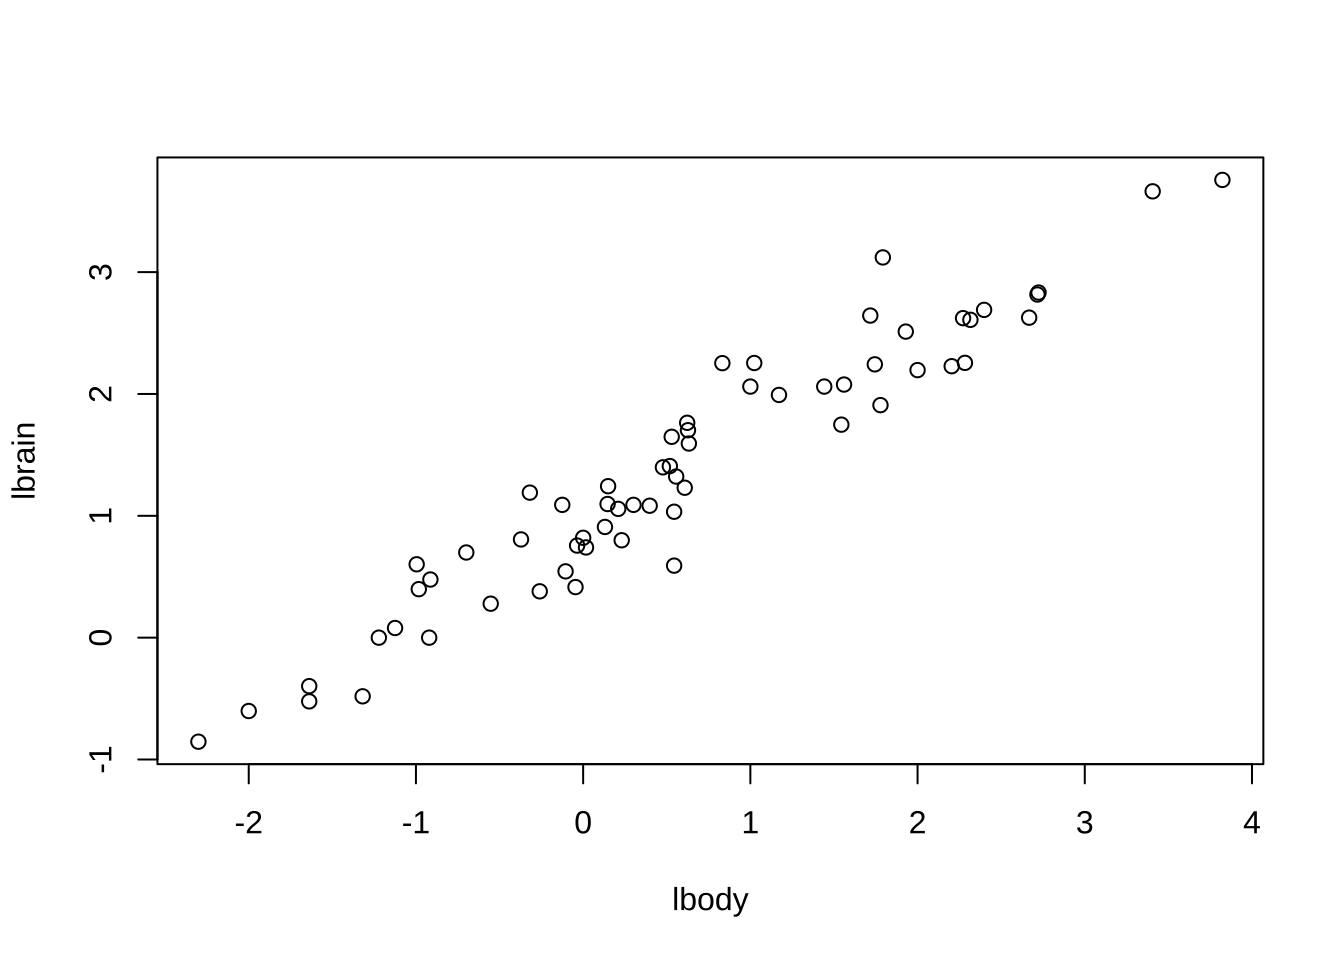
\includegraphics{lmbook_files/figure-latex/unnamed-chunk-6-1.pdf}

위와 같은 자료를 이용하여 자동차의 속도가 주어졌을 경우 제동거리를 예측하려고 한다면 어떤 방법을 사용해야 할까? 회귀분석(regression analysis)는 여러 개의 변수들의 함수적 관계를 분석하는 통계적 방법이다. 일반적으로 한 개 또는 여러 개의 설명변수들(explanatory variables)이 관심있는 반응변수(response variable)에 어떤 형태로 영향을 미치는지에 파악하고 설명변수와 반응변수의 함수 관계를 통계적으로 추론하는 것이 회귀분석의 목적이다.

위의 예제에서 자동차의 속도를 \(x\) 라고 하고 제동거리를 \(y\) 라고 하면 다음과 같은 선형식으로 자동차의 속도와 제동거리의 관계를 나타내는 것을 선형회귀식(linear regression function) 또는 선형예측식(linear predictor)이라고 한다.

\begin{equation} 
E(y|x) = \beta_0 + \beta_1 x
\label{eq:linreg01}
\end{equation}

식 \eqref{eq:linreg01}은 반응변수 \(y\)의 \textbf{평균}이 설명변수 \(x\) 의 선형식(linear function)으로 나타나는 관계를 가정한 것이며 절편 \(\beta_0\) 와 기울기 \(\beta_1\) 는 자료를 통하여 추정해야 한다.

위에서 본 \texttt{cars} 예제와 같이 \(n\) 개의 자료 \((x_1,y_1),(x_2,y_2),..,(x_n, y_n)\)을 독립적으로 추출하였다면 자료의 생성 과정을 다음과 같은 단순 선형회귀 모형(simple linear regression model)로 나타낸다. 반응변수 \(y_i\)는 설명변수 \(x_i\)의 선형함수로 표현된 선형 예측식 \eqref{eq:linreg01}과 임의의 오차항 (random error) \(e_i\) 의 합으로 나타내어진다.

\begin{equation} 
y_i = E(y_i | x_i) + e_i = \beta_0 + \beta_1 x_i + e_i, \quad i=1,2,\dots,n
\label{eq:linreg02}
\end{equation}

위 \eqref{eq:linreg02}에서 \(\beta_0\)와 \(\beta_1\)은 회귀계수(regression coefficient)라고 하며 주어진 자료를 이용하여 추정해야할 모수이다.

오차항 \(e_i\)는 평균이 \(0\)이고 분산이 \(\sigma^2\) 인 임의의 확률분포를 따르며 서로 독립이라고 가정한다.\\
\[ E(e_i)=0, \quad V(e_i) = \sigma^2 \quad i=1,2,\dots,n \]
오차항의 분산 \(\sigma^2\)도 추정해야할 모수(parameter)이다.

\hypertarget{lse}{%
\subsection{최소제곱법}\label{lse}}

앞에서 언급한 것과 같이 선형회귀모형 \eqref{eq:linreg02}에서 모수 \(\beta_0\)와 \(\beta_1\)를 회귀계수라고 하며 자료를 이용하여 추정해야 한다.
\(n\)개의 자료를 이용하여 회귀계수 \(\beta_0\)와 \(\beta_1\)를 추정하려고 할 때 사용할 수 있는 방법들 중에서 가장 쉽고 유용한 방법은 최소제곱법(least square method)이다.

회귀모형 \eqref{eq:linreg02}에서 \(\beta_0\)와 \(\beta_1\)의 값이 주어졌다면 설명변수 \(x_i\) 에서 반응변수의 관측값 \(y_i\)에 가장 합리적인 예측값은 무었일까?
가장 합리적인 예측값은 주어진 \(x_i\)에서 반응변수의 평균값인 \(E(y_i | x_i)=\beta_0 + \beta_1 x_i\)이다. 여기서 실제 관측하여 얻어진 값 \(y_i\)와 예측값 \(\beta_0 + \beta_1 x_i\) 사이에는 오차에 의해서 차이가 발생할 수 있다. 그 차이를 잔차(residual)라고 하며 \(r_i\) 라고 표기한다.

\[  r_i = y_i - E(y_i|x_i) = y_i - (  \beta_0 +  \beta_1 x_i) \]

잔차는 위에 식에서 알 수 있듯이 관측값과 회귀식을 통한 예측값의 차이를 나타낸 것이다. 그러면 자료를 가장 잘 설명할 수 있는 회귀직선을 얻기 위해서는 잔차 \(r_i\)를 가장 작게하는 회귀모형을 세워야 한다. 잔차들을 최소로 하는 방법들 중 하나인 최소제곱법은 잔차들의 제곱합을 최소로 하는 회귀계수 \(\beta_0\)와 \(\beta_1\)를 추정하는 방법이다. 잔차들의 제곱합은 다음과 같이 표현된다.

\begin{equation} 
 S(\beta_0 , \beta_1) = \sum^n_{i=1}r^2_i = \sum^n_{i=1}[y_i-(\beta_0 + \beta_1 x_i)]^2 
 \label{eq:rsq}
 \end{equation}

\begin{rmdnote}
식 \eqref{eq:rsq} 를 잔차제곱합(residusl sum of square)이라고 부른다. 일반적으로 회귀계수의 값이 특정지어져서 실제로 잔차를 계산할 수 있는 경우 잔차제곱합이라고 부른다. 뒤에 분산분석에서는 잔차제곱합을 SSE(sum of square error)라고 부른다.

잔차제곱합을 최소로 하는 회귀계수의 값을 찾는 최적화의 목표로 잔차제곱합이 제시될 때 이를 오차제곱합(error sum of square)이라고 부른다.
\end{rmdnote}

위의 오차제곱합 \(S(\beta_0 , \beta_1)\) 을 최소화하는 \(\beta_0\)와 \(\beta_1\)의 값을 구하는 방법은 오차제곱합이 \(\beta_0\)와 \(\beta_1\)의 미분 가능한 2차 함수이고 아래로 볼록한 함수(convex function)임을 이용한다.

\begin{Shaded}
\begin{Highlighting}[]
\NormalTok{gridnum }\OtherTok{\textless{}{-}} \DecValTok{60}
\NormalTok{sizing }\OtherTok{\textless{}{-}} \DecValTok{5}
\NormalTok{extrascale }\OtherTok{\textless{}{-}} \DecValTok{10}
\NormalTok{extrascale2 }\OtherTok{\textless{}{-}} \FloatTok{0.7}
\NormalTok{b0 }\OtherTok{\textless{}{-}} \FunctionTok{seq}\NormalTok{(}\SpecialCharTok{{-}}\FloatTok{17.6}\SpecialCharTok{{-}}\NormalTok{sizing}\SpecialCharTok{*}\NormalTok{extrascale,  }\SpecialCharTok{{-}}\FloatTok{17.6}\SpecialCharTok{+}\NormalTok{sizing}\SpecialCharTok{*}\NormalTok{extrascale, }\AttributeTok{length=}\NormalTok{gridnum )}
\NormalTok{b1 }\OtherTok{\textless{}{-}} \FunctionTok{seq}\NormalTok{(}\DecValTok{4}\SpecialCharTok{{-}}\NormalTok{sizing}\SpecialCharTok{*}\NormalTok{extrascale2, }\DecValTok{4}\SpecialCharTok{+}\NormalTok{sizing}\SpecialCharTok{*}\NormalTok{extrascale2, }\AttributeTok{length=}\NormalTok{gridnum )}

\NormalTok{SSE }\OtherTok{\textless{}{-}} \FunctionTok{matrix}\NormalTok{(}\DecValTok{0}\NormalTok{, gridnum, gridnum )}
\ControlFlowTok{for}\NormalTok{ (i }\ControlFlowTok{in} \DecValTok{1}\SpecialCharTok{:}\NormalTok{gridnum ) \{}
  \ControlFlowTok{for}\NormalTok{ (j }\ControlFlowTok{in} \DecValTok{1}\SpecialCharTok{:}\NormalTok{gridnum )\{}
\NormalTok{    r }\OtherTok{\textless{}{-}}\NormalTok{ cars}\SpecialCharTok{$}\NormalTok{dist}\SpecialCharTok{{-}}\NormalTok{ b0[i] }\SpecialCharTok{{-}}\NormalTok{b1[j]}\SpecialCharTok{*}\NormalTok{cars}\SpecialCharTok{$}\NormalTok{speed}
\NormalTok{    SSE[i,j]  }\OtherTok{\textless{}{-}}\NormalTok{ (}\FunctionTok{sum}\NormalTok{(r}\SpecialCharTok{\^{}}\DecValTok{2}\NormalTok{))}\SpecialCharTok{/}\DecValTok{1000}
\NormalTok{  \}}
\NormalTok{\}}

\FunctionTok{persp3D}\NormalTok{(b0, b1, SSE, }\AttributeTok{theta =}\DecValTok{30}\NormalTok{, }\AttributeTok{phi =} \DecValTok{20}\NormalTok{, }\AttributeTok{expand =} \DecValTok{1}\NormalTok{)}
\end{Highlighting}
\end{Shaded}

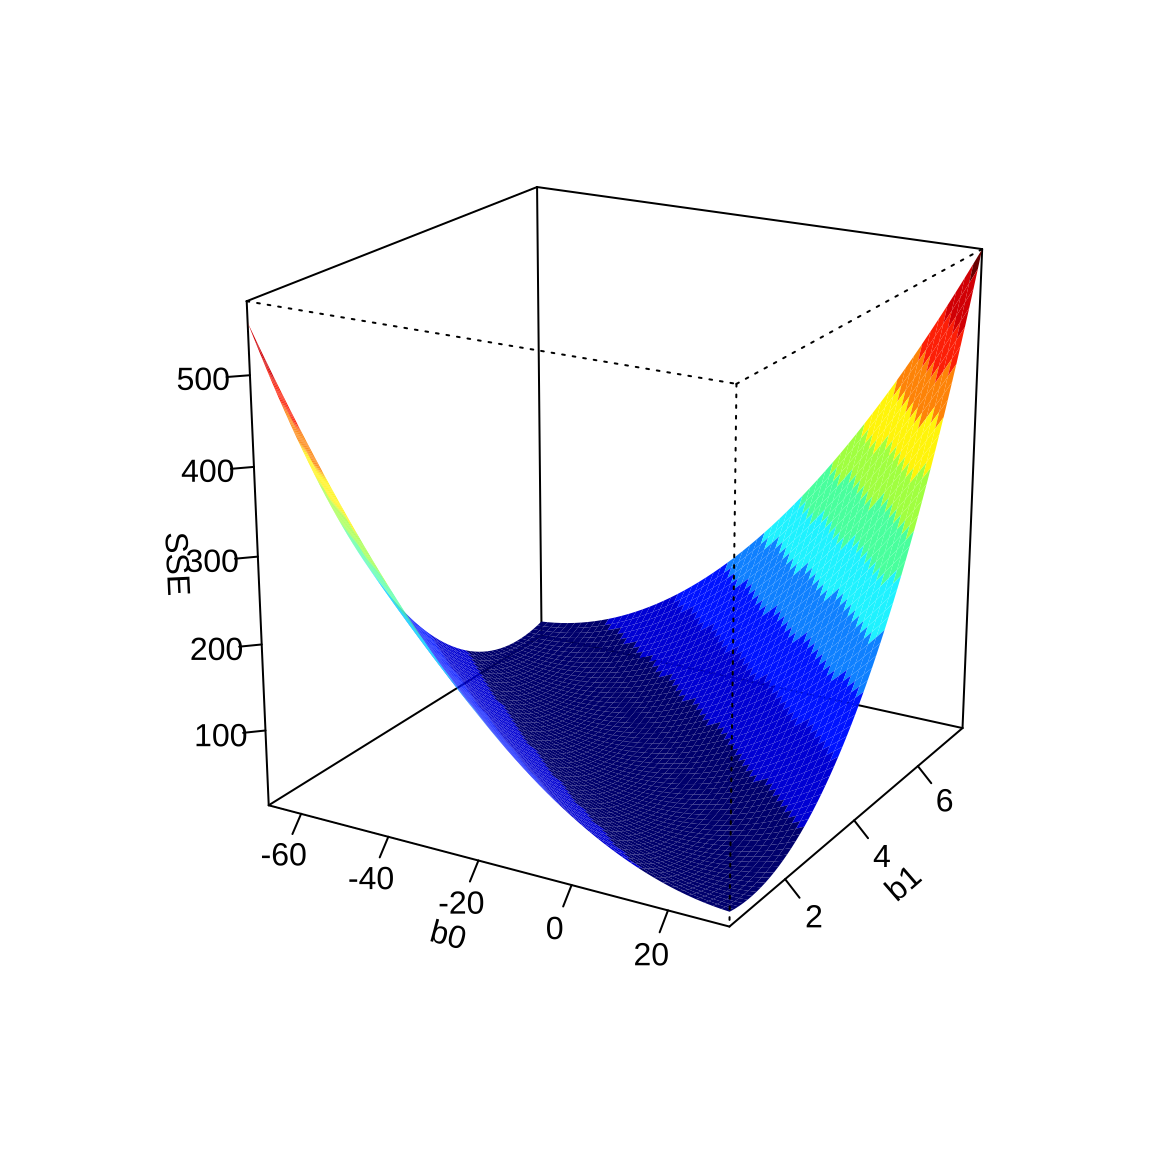
\includegraphics{lmbook_files/figure-latex/unnamed-chunk-8-1.pdf}

\begin{Shaded}
\begin{Highlighting}[]
\CommentTok{\# SSE의 그림을 쉽게 그리기 위하여 변수들을 표준화!}
\NormalTok{std\_cars }\OtherTok{\textless{}{-}} \FunctionTok{as.data.frame}\NormalTok{(}\FunctionTok{scale}\NormalTok{(cars))}
\NormalTok{gridnum }\OtherTok{\textless{}{-}} \DecValTok{60}
\NormalTok{sizing }\OtherTok{\textless{}{-}} \DecValTok{1}
\NormalTok{b0 }\OtherTok{\textless{}{-}} \FunctionTok{seq}\NormalTok{(}\DecValTok{0}\SpecialCharTok{{-}}\NormalTok{sizing,  }\DecValTok{0}\SpecialCharTok{+}\NormalTok{sizing, }\AttributeTok{length=}\NormalTok{gridnum )}
\NormalTok{b1 }\OtherTok{\textless{}{-}} \FunctionTok{seq}\NormalTok{(}\DecValTok{1}\SpecialCharTok{{-}}\NormalTok{sizing, }\DecValTok{1}\SpecialCharTok{+}\NormalTok{sizing, }\AttributeTok{length=}\NormalTok{gridnum )}

\NormalTok{SSE }\OtherTok{\textless{}{-}} \FunctionTok{matrix}\NormalTok{(}\DecValTok{0}\NormalTok{, gridnum, gridnum )}
\ControlFlowTok{for}\NormalTok{ (i }\ControlFlowTok{in} \DecValTok{1}\SpecialCharTok{:}\NormalTok{gridnum ) \{}
  \ControlFlowTok{for}\NormalTok{ (j }\ControlFlowTok{in} \DecValTok{1}\SpecialCharTok{:}\NormalTok{gridnum )\{}
\NormalTok{    r }\OtherTok{\textless{}{-}}\NormalTok{ std\_cars}\SpecialCharTok{$}\NormalTok{dist}\SpecialCharTok{{-}}\NormalTok{ b0[i] }\SpecialCharTok{{-}}\NormalTok{b1[j]}\SpecialCharTok{*}\NormalTok{std\_cars}\SpecialCharTok{$}\NormalTok{speed}
\NormalTok{    SSE[i,j]  }\OtherTok{\textless{}{-}} \FunctionTok{sum}\NormalTok{(r}\SpecialCharTok{\^{}}\DecValTok{2}\NormalTok{)}
\NormalTok{  \}}
\NormalTok{\}}
\FunctionTok{persp3D}\NormalTok{(b0, b1, SSE, }\AttributeTok{theta =}\DecValTok{40}\NormalTok{, }\AttributeTok{phi =} \DecValTok{15}\NormalTok{, }\AttributeTok{expand =} \DecValTok{1}\NormalTok{)}
\end{Highlighting}
\end{Shaded}

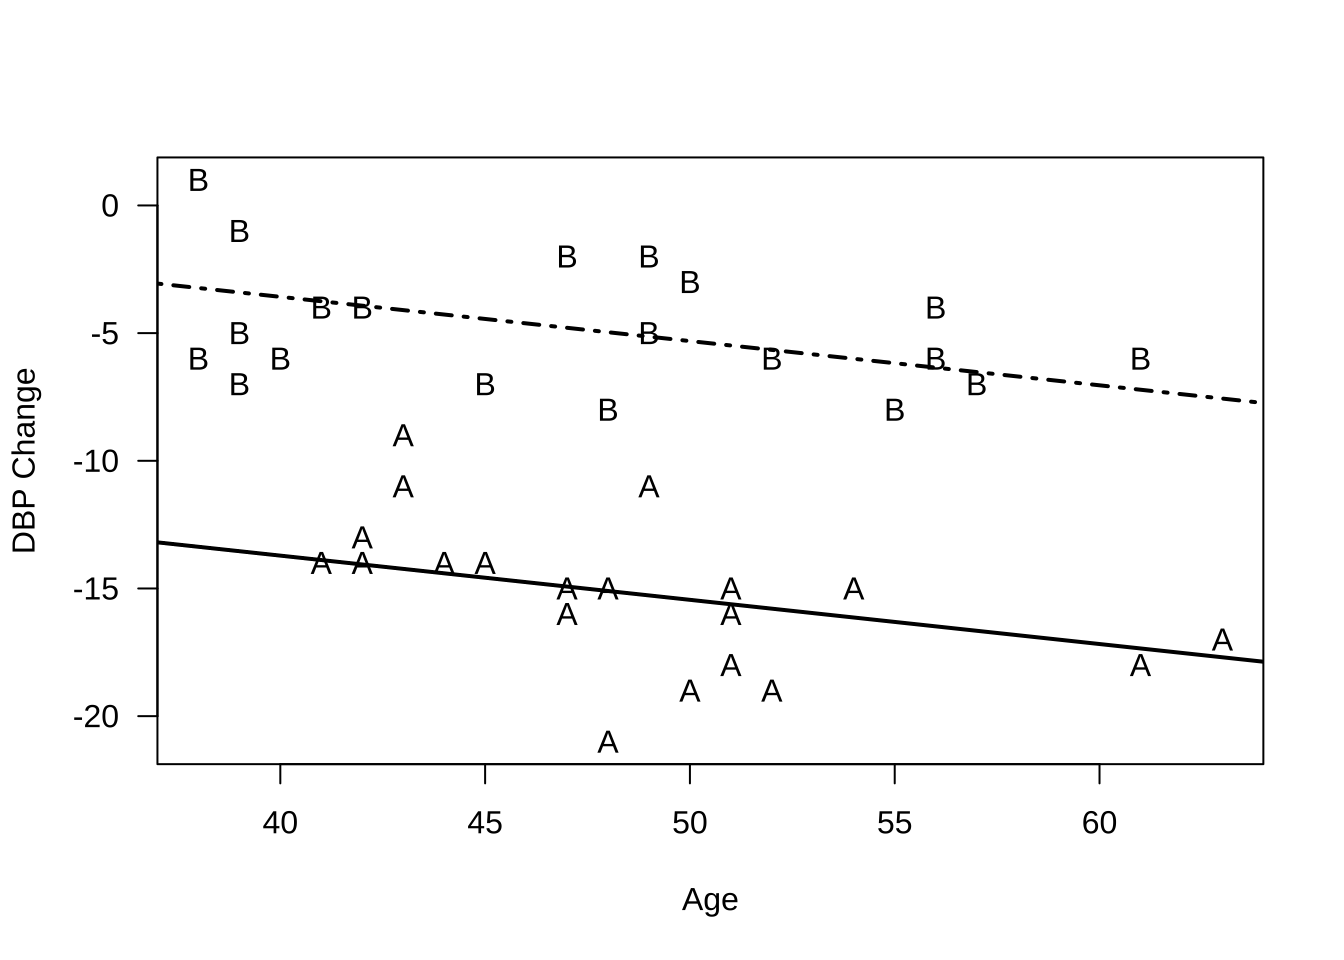
\includegraphics{lmbook_files/figure-latex/unnamed-chunk-9-1.pdf}

오차제곱합을 각 회귀계수에 대해서 편미분을 하고 0으로 놓으면 아래와 같이 두 방정식이 얻어진다.

\begin{align}
 \pardiff{ S(\beta_0 , \beta_1)}{\beta_0} & = \sum^n_{i=1}(-2)[y_i-(\beta_0+\beta_1 x_i)]=0  \label{eq:normaleq01}  \\ 
\pardiff{ S(\beta_0 , \beta_1)}{\beta_1}  & = \sum^n_{i=1}(-2 x_i)[y_i-(\beta_0+\beta_1 x_i)]=0 \label{eq:normaleq02}
\end{align}
위의 연립방정식을 행렬식으로 표시하면 다음과 같이 나타낼 수 있다.

\[ 
\begin{bmatrix}
n & \sum_i x_i \\
\sum_i x_i & \sum_i x^2_i
\end{bmatrix}
\begin{bmatrix}
\beta_0 \\
\beta_1
\end{bmatrix}
=
\begin{bmatrix}
\sum_i y_i \\
\sum_i x_i y_i
\end{bmatrix}
\]

위의 방정식을 풀어서 구한 회귀계수의 추정치를 \(\hat \beta_0\), \(\hat \beta_1\) 이라고 하면 다음과 같이 주어진다.

\begin{align*}
 \hat \beta_0 &= \bar y - \hat \beta_1 \bar x  \\ 
  \hat \beta_1 &=  \frac{ \sum_i (x_i - \bar x)(y_i - \bar y)}{\sum_i (x_i - \bar x)^2} 
\end{align*}

최소제곱법에서 얻어진 회귀계수의 추정량 \(\hat \beta_0\)과 \(\hat \beta_1\) 을 이용한 반응변수 \(y_i\) 에 대한 예측값 \(\hat y_i\)는 다음과 같이 정의되고

\[ \hat y_i = \hat E(y_i|x_i) = \hat \beta_0 + \hat \beta_1 x_i \]

잔차 \(r_i\)는 다음과 같이 계산한다.

\[ r_i = y_i - (\hat \beta_0 + \hat \beta_1 x_i) = y_i -\hat y_i  \]

잔차 \(r_i\)는 다음과 같은 성질을 가진다.

\begin{enumerate}
\def\labelenumi{\arabic{enumi}.}
\tightlist
\item
  \(\sum_{i=1}^n r_i = 0\)
\item
  \(\sum_{i=1}^n x_i r_i = 0\)
\end{enumerate}

이제 위에서 본 \texttt{cars} 자료를 가지고 선형회귀모형 \eqref{eq:linreg02} 에 나타난 회귀계수를 추정해보자. 아래는 \texttt{R} 프로그램에서 함수 \texttt{lm}을 이용한 추정결과이다.

\begin{Shaded}
\begin{Highlighting}[]
\NormalTok{lmOut }\OtherTok{\textless{}{-}} \FunctionTok{lm}\NormalTok{(dist}\SpecialCharTok{\textasciitilde{}}\NormalTok{speed, }\AttributeTok{data=}\NormalTok{cars)}
\FunctionTok{summary}\NormalTok{(lmOut)}
\end{Highlighting}
\end{Shaded}

\begin{verbatim}
## 
## Call:
## lm(formula = dist ~ speed, data = cars)
## 
## Residuals:
##     Min      1Q  Median      3Q     Max 
## -29.069  -9.525  -2.272   9.215  43.201 
## 
## Coefficients:
##             Estimate Std. Error t value Pr(>|t|)    
## (Intercept) -17.5791     6.7584  -2.601   0.0123 *  
## speed         3.9324     0.4155   9.464 1.49e-12 ***
## ---
## Signif. codes:  0 '***' 0.001 '**' 0.01 '*' 0.05 '.' 0.1 ' ' 1
## 
## Residual standard error: 15.38 on 48 degrees of freedom
## Multiple R-squared:  0.6511, Adjusted R-squared:  0.6438 
## F-statistic: 89.57 on 1 and 48 DF,  p-value: 1.49e-12
\end{verbatim}

위에서 주어진 선형회귀모형 \eqref{eq:linreg02} 에 대한 추정 결과를 이용하면 자동차의 속도(\(x\) = \texttt{speed})와 제동거리(\(y\) = \texttt{dist})의 관계는 다음과 같은 회귀식으로 나타낼 수 있다.

\begin{Shaded}
\begin{Highlighting}[]
\NormalTok{equatiomatic}\SpecialCharTok{::}\FunctionTok{extract\_eq}\NormalTok{(lmOut, }\AttributeTok{use\_coefs =} \ConstantTok{TRUE}\NormalTok{)}
\end{Highlighting}
\end{Shaded}

\[
\operatorname{\widehat{dist}} = -17.58 + 3.93(\operatorname{speed})
\]

위의 추정식을 이용하면 주어진 자동차의 속도에서 제동거리를 예측할 수 있다. 예를 들어 자동차의 속도가 25 mph인 경우에는 제동거리의 평균이 80.73 mph 임을 알 수 있다.

\[ E(y|x=25) = −17.58 + 3.93 (25) = 80.73 \]

\begin{Shaded}
\begin{Highlighting}[]
\NormalTok{newcars }\OtherTok{\textless{}{-}} \FunctionTok{data.frame}\NormalTok{(}\AttributeTok{speed =} \FunctionTok{c}\NormalTok{(}\DecValTok{25}\NormalTok{))}
\FunctionTok{predict}\NormalTok{(lmOut, }\AttributeTok{newdata=}\NormalTok{newcars)}
\end{Highlighting}
\end{Shaded}

\begin{verbatim}
##        1 
## 80.73112
\end{verbatim}

기울기의 추정값 \(\hat \beta_1 = 3.93\) 은 자동차의 속도 (\(x\))가 1 mph 증가할 때 평균 제동거리 (\(E(y|x)\))가 3.93 ft 증가한다는 의미이다.

\[ \hat E(y | x) = −17.58 + 3.93 x \]

\hypertarget{uxbaa8uxbd84uxc0b0uxc758-uxcd94uxc815uxacfc-uxacb0uxc815uxacc4uxc218}{%
\subsection{모분산의 추정과 결정계수}\label{uxbaa8uxbd84uxc0b0uxc758-uxcd94uxc815uxacfc-uxacb0uxc815uxacc4uxc218}}

최소제곱법을 통해서 회귀분석을 실시하였을때 우리는 적합된 회귀선이 얼마나 실제 관측값들을 잘
설명하고 있는지를 파악하는 것이 모형의 유용성을 판단하는데 중요한 작업이다. 즉, 적합된 회귀선이 관측값을 예측할 때의 변동성을 측정하는 것이 중요하다. 그 변동의 정도를 나타내는 것이 모분산 \(\sigma^2\)의 추정이다. 먼저 다음 평균제곱오차(mean residual sum of square; \(S^2\) 또는 MSE)를 정의하면 다음과 같다.

\begin{equation} 
S^2 = \frac{\sum r^2_i}{n-2} = \frac{\sum(y_i-\hat \beta_0 - \hat \beta_1 x_i)^2}{n-2}
 = \frac{\sum(y_i-\hat y_i)^2}{n-2} = \frac{SSE}{n-2} = MSE
\label{eq:rss}
\end{equation}

여기서 SSE는 잔차제곱합을 나타낸다. \(S^2\)은 모분산의 불편 추정량이다.

\[ E(s^2) = E(MSE) =\sigma^2 \]

모분산의 추정량이 작을수록 관측값 \(y\)의 변동 중 회귀식이 설명할 수 변동이 크다는 것을 나타낸다. 관측값들이 회귀식으로부터 멀리 떨어져 있으면 MSE는 커진다.

\[ \hat V ( \hat {\bm \beta }) = \hat \sigma^2 (\bm X^t \bm X)^{-1} = s^2(\bm X^t \bm X)^{-1} \]

모분산의 불편 추정량과 더불어 회귀식의 적합에 대한 기준으로서 결정계수(coefficient of determination; \(R^2\))가 있다. 결정계수는 적합의 정도(degree of fitting)를 측정한다. 즉 ``독립변수는 반응변수를 얼마나 잘 예측하느냐''에 대한 정도를 수치로 표현한 것이다. 독립변수가없고 반응변수 \(y\)만 존재한다고 하면 다음과 같은 모형을 생각할 수 있다.

\begin{equation}
y_i = \beta_0 +e_i, \quad e_i \sim (0,\sigma^2) 
\label{eq:meanmodel}
\end{equation}

회귀분석에서 독립변수와 반응변수 간에 전혀 회귀관계가 없다면 당연히 반응변수의 값은 독립변수 값의 변동 여하에 전혀 영향을 받지 않아야 한다. 단순회귀모형에서 독립변수 \(x\)의 값의 변화를 반응변수 \(y\)로 값으로 표현하는것이 바로 기울기 \(\beta_1\)이다.

독립변수와 반응변수 사이에 아무런 관계가 존재 하지 않는다면 \(\beta_1\)의 값은 0 이 될것이다. 이러한 경우 모형을 \eqref{eq:meanmodel} 과 같이 표현할 수 있으며 평균모형이라고 부른다.

이러한 평균 모형에 대한 최소제곱법을 적용하여 \(\beta_0\)의 추정량을 구하면 추정량 \(\hat \beta_0\)는 \(\bar y\)가 된다. 그 이유는 위의 모형에 오차제곱합을 구해보면 다음과 같은 형식이 된다
\[ S(\beta_0)=  \sum^n_{i=1}[y_i-\beta_0]^2 \]
여기서 \(\beta_0\)에 대하여 최고로 하는 지점을 찾아보면 다음과 같은 방정식을 얻을 수 있다.
\[ \frac{\partial S(\beta_0)}{\partial \beta_0}  = 0  \Rightarrow  \sum^n_{i=1}[y_i - \beta_0] = 0 \]
이 방정식을 풀면 \(\hat \beta_0 = \bar y\)가 됨을 알 수 있다.
결국 독립변수가 반응변수에 아무른 영향을 주지못하게 되면 \(y\)의 예측값은 평균 \(\bar y\)임을 알 수 있다 (평균모형 \eqref{eq:meanmodel} 경우 \(\bar y\)는 \(\beta_0\) 의 최소제곱추정량이다).

관측값이 가지고 있는 변동은 \(y_i - \bar y\)로 나타낼 수 있으며 회귀식에 예측치 \(\hat y_i=\hat \beta_0 + \hat \beta_1 x_i\)를 고려하면 관측값의 변동을 다음과 같이 분해할 수 있다.

\[ (y_i - \bar y) = (y_i - \hat y_i) + (\hat y_i - \bar y) \]

즉, (실제값과 평균 간 차이)=(실제값과 예측값 간의 차이(잔차))+(예측값과 평균 간 차이)이다. 이 부분에서 잔차는 작으면 작을수록 회귀 적합이 잘 되었다고 할 수 있다. 이때 \(y_i - \bar y\)을 모두 합한 값은 0이 되므로 총 변동을 제곱합 형태로 표현하면 다음과 같다.

\begin{eqnarray*}
 \sum^n_{i=1}(y_i - \bar y)^2 &= & \sum^n_{i=1}[(y_i-\hat y_i)+(\hat y_i - \bar y)]^2 \\
 &=& \sum^n_{i=1}(y_i-\hat y_i)^2+\sum^n_{i=1}(\hat y_i - \bar y)^2
        + 2\sum^n_{i=1}(y_i-\hat y_i)(\hat y_i-\bar y)  \\
 &=& \sum^n_{i=1}(y_i-\hat y_i)^2+\sum^n_{i=1}(\hat y_i - \bar y)^2 + 0 \quad \text{(why?)}
 \end{eqnarray*}

따라서 다음과 같은 제곱합의 분해를 얻게 된다.

\[ \sum^n_{i=1}(y_i - \bar y)^2 = \sum^n_{i=1}(y_i-\hat y_i)^2+\sum^n_{i=1}(\hat y_i - \bar y)^2\]
여기서 총제곱합(total sum of square; SST)와 모형제곱합(regression sum of square; SSR)를 다음과 같이 정의하면
\[ SST =  \sum^n_{i=1}(y_i - \bar y)^2, \quad  SSR = \sum^n_{i=1}(\hat y_i-\bar y_i)^2 \]

총제곱합은 잔차제곱합 과 모형제곱합으로 분해되며

\[ SST = SSE + SSR \]

관측값들이 보여주는 총 변동인 총제곱합(SST)에서 회귀모형으로 설명할 수 있는 변동, 즉 모형제곱합(SSR)이 차지하는 비율을 결정계수(coefficient of determination)라 하며 \(R^2\)으로 표현한다.

\[ R^2 = \frac{SSR}{SST} =  1 -\frac{SSE}{SST}  =1- \frac{\sum^n_{i=1}(y_i-\hat y_i)^2}{ \sum^n_{i=1}(y_i - \bar y)^2} \]

위의 식에서 보면 잔차제곱합(SSE)가 상대적으로 작아질수록 결정계수가 커진다.
결정계수 \(R^2\)는 언제나 0 이상 1 이하의 값을 갖는다. 회귀모형이 데이터에 아주 잘 적합되면 결정계수의 값은 1 에 가깝게 된다.

\hypertarget{uxc911uxd68cuxadc0-uxbaa8uxd615}{%
\section{중회귀 모형}\label{uxc911uxd68cuxadc0-uxbaa8uxd615}}

일반적으로 회귀모형에서 반응변수의 수는 하나인 경우가 많지만 설명변수의 수는 여러 개인 경우가 많다. 이런 경우 중선형 회귀 모형(multiple linear regression)은 다음과 같이 표현할 수 있고, \(p\)개의 설명변수가 있다고 가정하고 \((x_1, x_2, \cdots, x_p)\) 표본의 크기 \(n\)인 자료가 얻어지면 선형회귀식을 행렬로 다음과 같이 표현할 수 있다.

\begin{equation*}
y_i = \beta_0 + \beta_1 x_{i1} + \beta_2 x_{i2} + \cdots + \beta_p x_{ip} +  e_i = \bm x^t_i \bm \beta +  e_i 
\end{equation*}

위의 식을 다시 표현하면 다음과 같이 쓸 수 있다.

\[ 
y_i  = \bm x^t_i \bm \beta  + e_i  =
\begin{bmatrix}
1 & x_{i1} & x_{i2} & \cdots & x_{ip}
\end{bmatrix}
\begin{bmatrix}
\beta_{0} \\
\beta_{1} \\
\beta_{2} \\
\vdots \\
\beta_{p}
\end{bmatrix}
+ e_i
\]

이제 \(n\)개의 관측치 \(y_1,y_2, \dots, y_n\) 으로 이루어진 관측값 벡터 \(\bm y\)를 고려하면 n개의 관측치에 대한 회귀식을 행렬식으로 다음과 같이 표현할 수 있다.

\[ 
\begin{bmatrix}
y_{1} \\
y_{2} \\
\vdots \\
y_{n}
\end{bmatrix} =
\begin{bmatrix}
1 & x_{11} & \cdots & x_{1p} \\
1 & x_{21} & \cdots & x_{2p} \\
\vdots & \vdots & \vdots & \vdots \\
1 & x_{n1} & \cdots & x_{np}
\end{bmatrix}
\begin{bmatrix}
\beta_{0} \\
\beta_{1} \\
\vdots \\
\beta_{p}
\end{bmatrix}
+
\begin{bmatrix}
 e_{1} \\
 e_{2} \\
\vdots \\
 e_{n}
\end{bmatrix}
\]

위의 식을 간단히 행렬식으로 표시하면 다음과 같다.

\begin{equation} 
\bm y = \bm X \bm \beta + \bm e
\label{eq:multireg2}
\end{equation}

위의 행렬식에서 각 벡터와 행렬의 차원은 다음과 같다.

\begin{itemize}
\tightlist
\item
  \(\bm y\): \(n \times 1\)
\item
  \(\bm X\): \(n \times (p+1)\)
\item
  \(\bm \beta\): \((p+1) \times 1\)
\item
  \(\bm e\): \(n \times 1\)
\end{itemize}

여기서 회귀분석의 오차항 \(e_i\)은 서로 독립이고 동일한 분산을 갖는다. 즉, 오차항은 다음의 분포를 따른다.
\[ \bm e  \sim (\bm 0,\sigma^2 \bm I_n) \]

따라서 관측값 벡터 \(\bm y\)의 평균은 다음과 같고

\begin{equation}
 E(\bm y|\bm X) = E(\bm X \bm \beta+\bm e)= \bm X \bm \beta + E(\bm e) = \bm X \bm \beta
\label{eq:multiregmean}
\end{equation}

\(\bm y\)의 분산은 아래와 같이 주어진다.

\begin{equation}
 V( \bm y| \bm X) = E[( \bm y -  \bm X \bm \beta)( \bm y -  \bm X \bm \beta)^t] = E( \bm  e   \bm  e^t) = \sigma^2 \bm I_n
\label{eq:multiregvar}
\end{equation}

여기서 오차항이 정규분포를 따른다면

\[ \bm  e   \sim N(\bm 0,\sigma^2 \bm I_n) \]

관측값 벡터 \(\bm y\) 또한 정규분포를 따른다

\[  \bm y \sim N( \bm X \bm \beta, \sigma^2 \bm I_n) \]

\hypertarget{uxcd5cuxc18cuxc81cuxacf1uxcd94uxc815}{%
\subsection{최소제곱추정}\label{uxcd5cuxc18cuxc81cuxacf1uxcd94uxc815}}

최소제곱추정법(least square estimation)은 자료의 관계을 잘 반영하는 회귀식을 구한 다음 실제 관측값 \(y_i\)과 예측값 \(\bm x_i^t \bm \beta\) 간에 차이인 잔차를 가장 작게 만드는 것이 목적이다. 모든 잔차항의 제곱의 합을 최소화하는 방법을 최소제곱법이라고 하며 이를 이용하여 회귀계수의 추정량을 찾는다.

\begin{equation} 
 \min_{\bm \beta} \sum_{i=1}^n (y_i -  \bm x_i^t \bm \beta )^2 = \min_{\bm \beta } ( \bm y -  \bm X \bm \beta )^t( \bm y -  \bm X \bm \beta ) 
 \label{eq:rsq2}
 \end{equation}

\hypertarget{uxbc29uxbc95-1}{%
\subsection{방법 1}\label{uxbc29uxbc95-1}}

\(\hat {\bm \beta}\)는 잔차의 제곱합 \eqref{eq:rsq2} 을 최소로 하는 최소제곱 추정량이다. 잔차의 제곱합을 \(S( \bm \beta)\)이라고 하면

\begin{align} 
S( \bm \beta ) & =  ( \bm y -  \bm X \bm \beta)^t( \bm y -  \bm X \bm \beta ) \notag \\
  & = \bm y^t \bm y - \bm y^t \bm X \bm \beta - \bm \beta^t \bm X^t \bm y
    + \bm \beta^t \bm X^t \bm X \bm \beta \notag \\
  & = \bm y^t \bm y -2  \bm \beta^t \bm X^t \bm y
    + \bm \beta^t \bm X^t \bm X \bm \beta \label{eq:rsq3}   
\end{align}

여기서 \(S( \bm \beta)\)를 최소로 하는 회귀계수벡터의 값을 구하기 위하여 \(S( \bm \beta)\)를 회귀계수벡터 \(\bm \beta\)로 미분한후 \(\bm 0\) 으로 놓고 선형 방정식을 풀어야 한다.

앞 절에 나오는 벡터미분을 이용하면

\begin{align*}
 \pardiff{ S( {\bm \beta})}{\bm \beta} & = 
 \pardiff{}{\bm \beta} (\bm y^t \bm y -2  \bm \beta^t \bm X^t \bm y
    + \bm \beta^t \bm X^t \bm X \bm \beta) \\
 & = \bm 0 -2 \bm X^t \bm y + 2 \bm X^t \bm X \bm \beta \\
 & =\bm 0
 \end{align*}

최소제곱 추정량을 구하기 위한 정규방정식은 다음과 같이 쓸 수 있다.

\begin{equation} 
 \bm X^t \bm X \bm \beta =  \bm X^t \bm y
 \label{eq:lsequation}
\end{equation}

방정식 \eqref{eq:lsequation}를 정규방정식(normal equation)이라고 한다. 만약 \(\bm X^t \bm X\)가 정칙행렬일 경우 최소제곱법에 의한 회귀계수 추정량 \(\hat {\bm \beta}\) 다음과 같다.

\begin{equation}
  \hat {\bm \beta} = ( \bm X^t \bm X)^{-1} \bm X^t \bm y
  \label{eq:lsestimator}
\end{equation}

예측값 벡터 \(\hat {\bm y}\) 는 \(E(\bm y | \bm X)\)의 추정치로서 다음과 같다.

\[ \hat E(\bm y | \bm X)= \hat {\bm y} = \bm X \hat {\bm \beta} = \bm  X(\bm X^t \bm X)^{-1} \bm X^t y \]

만약 \(\bm X^t \bm X\)가 정칙행렬이 아닐 경우 최소제곱법에 의한 회귀계수 추정량 \(\hat {\bm \beta}\)은 \(\bm X^t \bm X\)의 일반화 역행렬 \((\bm X^t \bm X)^-\)를 이용하여 다음과 같이 구한다. 이 경우 일반화 역행렬이 유일하지 않기 때문에 회귀계수 추정량도 유일하지 않다.

\[
  \hat {\bm \beta} = ( \bm X^t \bm X)^{-} \bm X^t \bm y
\]

\hypertarget{uxbc29uxbc95-2}{%
\subsection{방법 2}\label{uxbc29uxbc95-2}}

식 \eqref{eq:rsq2}에서 나오는 오차벡터를 정의하고 \(\bm e = (\bm y - \bm X \bm \beta)\) 오차벡터를
모수벡터 \(\bm \beta\)로 미분하면 다음과 같은 결과를 얻는다.

\[ \pardiff{\bm e}{\bm \beta} = \pardiff{ (\bm y - \bm X \bm \beta)}{ \bm \beta} =
- \pardiff{ \bm X \bm \beta}{ \bm \beta} \equiv
- \pardiff{\bm \beta^t \bm X^t }{\bm \beta} = -\bm X^t \]

이제 오차제곱합 \(S( {\bm \beta})=\bm e^t \bm e\) 를 모수벡터로 미분하면 이차형식의 미분공식과
합성함수 미분공식을 차례로 적용하면 된다.
\[  \pardiff{ S( {\bm \beta})}{\bm \beta}=\pardiff{\bm e^t \bm e}{\bm \beta} =  \pardiff{\bm e }{\bm \beta} \pardiff{\bm e^t  \bm e}{\bm e} = -\bm X^t \left( 2 \bm e \right ) = -2 \bm X^t (\bm y - \bm X \bm \beta)  \]

위의 방정식을 \(\bm 0\)으로 놓으면 최소제곱 추정량 (열)벡터를 구한다.
\[ \bm X^t \bm y - \bm X^t  \bm X \bm \beta = \bm 0 \quad \rightarrow \quad
\hat{\bm \beta}  = (\bm X^t  \bm X)^{-1} \bm X^t  \bm y \]

\hypertarget{uxcd5cuxc18cuxc81cuxacf1-uxcd94uxc815uxb7c9uxc758-uxbd84uxd3ec}{%
\subsection{최소제곱 추정량의 분포}\label{uxcd5cuxc18cuxc81cuxacf1-uxcd94uxc815uxb7c9uxc758-uxbd84uxd3ec}}

회귀선을 추정하기 위한 회귀계수 추정값인 \(\bm b\)의 분포를 알아보기 위해서 우선 선형추정량을 보면 다음과 같다.

\[ \bm \beta = (\bm X^t\bm X)^{-1}\bm X' \bm y \equiv  \bm M \bm y \]
따라서 최소제곱 추정량은 관측값들의 선형 변환이다.
회귀계수 추정값 \(\bm \beta\)의 기대값은
\begin{eqnarray*}
 E( \bm \beta) &=& E( \bm M \bm y) = E(( \bm X^t \bm X)^{-1} \bm X' \bm y) \\
 &=& ( \bm X^t \bm X)^{-1} \bm X'E( \bm y) \\
 &=& ( \bm X^t \bm X)^{-1} \bm X^t \bm X \bm \beta \\
  &=& \bm \beta
\end{eqnarray*}

따라서 최소제곱 추정량 \(\bm \beta\)는 \(\beta\)의 불편추정량이다. 최소제곱 추정량 \(\bm \beta\)의 공분산 행렬을 전개해보면
\begin{eqnarray*}
 Var(\bm \beta) &=& Var(( \bm X^t \bm X)^{-1} \bm X^t \bm y) \\
&=& ( \bm X^t \bm X)^{-1} \bm X^t ~ Var( \bm y) ~ \bm X ( \bm X^t \bm X)^{-1} \\
&=&( \bm X^t \bm X)^{-1} \bm X^t[\sigma^2  \bm I_n] \bm X( \bm X^t \bm X)^{-1} \\
&=& \sigma^2( \bm X^t \bm X)^{-1} \bm X^t \bm X( \bm X^t \bm X)^{-1} \\
&=& \sigma^2( \bm X^t \bm X)^{-1} \\
\end{eqnarray*}

위에서 최소제곱 추정량의 평균과 공분산을 구할 때에는 정규성 가정이 필요하지않다. 만일 \(\bm y\)가 정규분포를 따른다면 \(\bm y\)의 선형변환으로부터 얻어진 \(\bm \beta\)의 분포는 정규분포이먀 다음과 같다.

\[  \bm \beta \sim N \left (\bm \beta, \sigma^2( \bm X^t \bm X)^{-1} \right ) \]

\hypertarget{uxac00uxc6b0uxc2a4-uxc815uxb9ac}{%
\section{가우스 정리}\label{uxac00uxc6b0uxc2a4-uxc815uxb9ac}}

\begin{theorem}
\protect\hypertarget{thm:unnamed-chunk-13}{}{\label{thm:unnamed-chunk-13} }선형회귀모형 \(\bm y = \bm X \bm \beta + \bm e\)에서 \(E( \bm e)=0, Var( \bm e)=\sigma^2 \bm I\)이 성립하면 최소제곱 추정량

\[ \hat{\bm \beta}=(\bm X^t \bm X)^{-1} \bm X^t \bm y\]

는 \(\bm \beta\)의 최소분산 선형 불편추정량이다.
\end{theorem}

위의 정리를 Gauss-Markov 정리라고 하며 이는 회귀계수 \(\bm \beta\)의 모든 선형 불편 추정량들 중에 최소제곱 추정량 \(\hat {\bm \beta}=(\bm X^t \bm X)^{-1} \bm X^t \bm y\)이 가장 작은 분산을 가짐을 뜻한다 (Best Linear Unbiased Estimator; BLUE).

Gauss-Markov 정리를 정확하게 표현하면 \(E(\bm L \bm y) = \bm \beta\)를 만족하는 모든 \(n \times n\) 차원의 행렬 \(\bm L\)과 임의의 벡터 \(\bm c\)에 대하여 다음이 성립한다.

\[ V(\bm c^t \hat {\bm \beta}) \le V(\bm c^t \bm L \bm y)  \]

Gauss-Markov 정리를 증명해보자. 관측벡터 \(\bm y\)에 대한 임의의 선형 추정량 \(\bm \beta^* = \bm L \bm y\)를 생각해보면 다시 다음의 형태로 표시할 수 있다.
\[  \bm \beta^* =  \bm L  \bm y = (\bm M + \bm L -\bm M ) \bm y = ( \bm M +  \bm A)  \bm y \]
여기서 \(\bm M = ( \bm X^t \bm X)^{-1} \bm X^t\) 이고 \(\bm A= \bm L- \bm M\) 이다.
임의의 선형 추정량 \(\bm \beta^*\)가 불편 추정량일 조건을 구해보자
\begin{align*}
 E( \bm \beta^*) & = E[( \bm M+ \bm A) \bm y] \\
            & = ( \bm M+ \bm A)E( \bm y) \\
            & = ( \bm M+ \bm A)X \bm \beta \\
            & = ( \bm X^t  \bm X)^{-1} \bm X^t  \bm X  \bm \beta +  \bm A  \bm X  \bm \beta \\
            & =  \bm \beta+AX \bm \beta\\
\end{align*}
여기서 불편추정량이 되기 위해서는 \(E( \bm \beta^*)= \bm \beta\) 조건을 만족 해야되며 따라서 \(\bm A \bm X=0\)이되어야한다 (이 조건은 \(\bm A=0\)를 의미하는 것은 아니다).

이제 최소분산을 가지기 위해서 \(\bm A \bm X=0\)을 만족하는 행렬 \(\bm A\)중에서 \(Var( \bm \beta^*)\)을 최소로하는 행렬 \(\bm A\)를 구해야 한다. \(\bm \beta^*\)의 공분산 행렬은 \(AX=0\)이므로
\begin{align*}
 V( \bm \beta^*) & = ( \bm M+ \bm A)V( \bm y)( \bm M+ \bm A)^t\\
            & = ( \bm M+ \bm A)\sigma^2 I_n( \bm M+ \bm A)^t\\
            & = \sigma^2 ( \bm M \bm M^t+ \bm A \bm M^t+ \bm M  \bm A^t+ \bm A  \bm A^t)\\
            & = \sigma^2 [ ( \bm X^t  \bm X)^{-1}  \bm X^t  \bm X( \bm X^t \bm X)^{-1} + \bm A  \bm X ( \bm X^t  \bm X)^{-1}+( \bm X^t  \bm X)^{-1} \bm X^t  \bm A^t+  \bm A  \bm A^t ]\\
            & = \sigma^2[( \bm X^t  \bm X)^{-1} +  \bm A  \bm A^t ]  \\
            & = V( \hat {\bm \beta} ) + \sigma^2 \bm A \bm A^t\\
\end{align*}

이제 임의의 벡터 \(\bm c\)에 대하여

\begin{align*}
 V( \bm c^t \bm \beta^*)  & = \bm c^t V (\bm \beta^*) \bm c \\
   & =  \bm c^t V( \hat {\bm \beta} ) \bm c + \sigma^2 \bm c^t \bm A \bm A^t \bm c \\
    & =  V( \bm c^t  \hat {\bm \beta} ) + \sigma^2 \bm c^t \bm A \bm A^t \bm c 
\end{align*}

다음이 성립하므로

\[ \bm c^t \bm A \bm A^t \bm c = \bm u^t \bm u = \sum_{i=1}^n u_i^2 \ge 0 \]

임의의 벡터 \(\bm c\)에 대하여

\[ V( \bm c^t \bm \beta^*) \ge  V( \bm c^t  \hat {\bm \beta} ) \]

이제 \(V( \bm c^t \bm \beta^*)\) 이 \(V( \bm c^t \hat {\bm \beta} )\)과 같으려면
다음 조건이 성립해야 하며

\[ \bm u = \bm c^t \bm A = \bm 0 \]

임의의 모든 벡터 \(\bm c\)에 대해서 위의 조건 성립해야 하므로 이는 \(\bm A = \bm 0\) 이 성립해야 한다. 또한 이조건은 \(\bm A \bm X=0\)도 만족 시켜준다. 따라서 \(\bm \beta\)의 최소분산 선형 불편추정량은 최소제곱법으로 구한 추정량이다.

여기서 주의할 점은 Gauss-Markov정리에서 관측값 \(\bm y\)에 대한 가정은 평균과 공분산의 가정만 주어졌으며 \(\bm y\)의 분포에 대한 가정이 없다. 참고로 만약에 \(\bm y\)가 정규분포를 따른다면 최소제곱 추정량은 최소분산 불편추정량이다.

\hypertarget{uxcd5cuxb300uxac00uxb2a5uxb3c4-uxcd94uxc815uxbc95}{%
\section{최대가능도 추정법}\label{uxcd5cuxb300uxac00uxb2a5uxb3c4-uxcd94uxc815uxbc95}}

관측값 벡터 \(\bm y\) 가 다음과 같이 선형모형이며 정규분포를 따른다고 가정하자.

\begin{equation}
\bm y \sim N( \bm X \bm \beta, \sigma^2 \bm I_n) 
\label{eq:normallm}
\end{equation}

선형모형 \eqref{eq:normallm}에 대한 가능도 함수는 다음과 같이 주어진다.

\begin{align*}
 L_n( \theta ;  y) & = L( \beta,\sigma^2|  y) \\
   & = \prod^n_{i=1} f(y_i)\\
   & = \prod^n_{i=1}(2 \pi \sigma^2)^{-\frac{1}{2}} \exp \left [-\frac{1}{2\sigma^2} (y_i- x_i^t \beta)^2 \right ] \\
   & = (2\pi\sigma^2)^{-\frac{n}{2}} \exp \left [ -\frac{1}{2\sigma^2}( y- X  \beta)^t( y- X  \beta) \right ]
\end{align*}

또한 분산에 대한 모수를 \(\tau=\sigma^2\) 과 같이 쓰면 로그 가능도함수는 다음과 같다.

\begin{align*}
\ell_n( \theta; y) & = -\frac{n}{2} \log (2 \pi)-\frac{n}{2} \log \sigma^2 -\frac { ( y- X  \beta)^t ( y- X  \beta) }{2\sigma^2} \\ 
   &= -\frac{n}{2} \log (2 \pi)-\frac{n}{2} \log \tau -\frac { ( y- X  \beta)^t ( y- X  \beta) }{2\tau}  
\end{align*}

이제 로그가능도함수로부터 구할 수 있는 스코어함수 \(s( \theta;y)\) 와 그에 대한 관측 피셔정보 \(J_n( \theta; y)\) 은 다음과 같이 주어진다.

\begin{align*}
s( \theta;  y) & =  \pardiff{}{ \theta}\ell_n( \theta;  y ) \\
  & =  \begin{bmatrix}
    \pardiff{}{ \beta}\ell_n( \theta;  y ) \\
    \pardiff{}{\tau}\ell_n( \theta;  y ) 
  \end{bmatrix} \\
  & = 
  \begin{bmatrix}
     X^t ( y- X  \beta)/\tau \\
    -\frac{n}{2\tau} +\frac { ( y- X  \beta)^t ( y- X  \beta) }{2\tau^2} 
  \end{bmatrix} \\
 J_n( \theta;  y) & =  -\pardiffdd{}{ \theta}{ \theta^t}\ell_n( \theta;y ) \\
  & = 
  - \begin{bmatrix}
    \pardiffdd{}{\beta}{ \beta^t}\ell_n( \theta;y ) & \pardiffdd{}{ \beta}{\tau^t}\ell_n( \theta;y )  \\
    \pardiffdd{}{\tau}{ \beta^t}\ell_n( \theta;y )  & \pardiffdd{}{\tau}{\tau^2}\ell_n( \theta;y ) 
  \end{bmatrix} \\
   & = 
  \begin{bmatrix}
      X^t  X /\tau &  - X^t ( y- X  \beta)/\tau^2   \\
    - X^t ( y- X  \beta)/\tau^2  &  - \frac{n}{2\tau^2} +\frac { ( y- X  \beta)^t ( y- X  \beta) }{\tau^3} 
  \end{bmatrix}
\end{align*}

\hypertarget{uxcd5cuxb300uxac00uxb2a5uxb3c4-uxcd94uxc815uxb7c9}{%
\subsection{최대가능도 추정량}\label{uxcd5cuxb300uxac00uxb2a5uxb3c4-uxcd94uxc815uxb7c9}}

이제 회귀계수 \(\beta\)에 대한 최대가능도 추정량은 스코어함수로 부터 얻어진 방정식 \(s( \theta; y)= 0\) 으로부터 얻어지며 다음과 같은 형태를 가진다.

\[ \hat { \beta} = ( X^t  X)^{-1}  X^t  y \]

\[   \hat \sigma^2 = \hat \tau = ( y- X  {\hat \beta})^t ( y- X  {\hat \beta})/n = \frac{SSE(\hat{ \beta})}{n} \]

여기서 유의할 점은 회귀계수 \(\beta\) 의 최대가능도 추정량은 최소제곱법으로 구한 추정량과 동일하다. 따라서 \(\hat { \beta}\)은 최소분산 불편 추정량이다. 하지만 오차항의 분산 \(\sigma^2\) 에 대한 최대가능도 추정량은 불편추정량이 아니다.

\[ E(\hat \sigma^2)  = E \left [ ( y- X  {\hat \beta})^t ( y- X  {\hat \beta})/n \right ] = E \left [ \frac{SSE}{n} \right ]  \ne \sigma^2 \]

참고로 오차항의 분산 \(\sigma^2\)에 대한 불편추정량은 \(SSE/(n-p)\)이다.

최대가능도 추정량의 점근적 분포를 이용하면 다음과 같이 말할 수 있다. 오차항이 정규분포인 선형모형인 경우 아래의 분포는 점근분포가 아닌 정확한 분포이다.

\[ \hat { \theta} -  \theta_0  \sim  N( 0,  I_n^{-1}( \theta_0)) \]

여기서

\[  I_n( \theta) = E[ J( \theta;  y)] =  
\begin{bmatrix}
      X^t X /\tau & 0   \\
    0  &   \frac{n}{2\tau^2} 
  \end{bmatrix}
\]
그리고
\[  I_n^{-1}( \theta) = 
\begin{bmatrix}
     \tau( X^t  X)^{-1}  & 0   \\
    0  &   \frac{2\tau^2}{n} 
  \end{bmatrix}
  = 
\begin{bmatrix}
     \sigma^2( X^t  X)^{-1}  & 0   \\
    0  &   \frac{2\sigma^4}{n} 
  \end{bmatrix}
\]

따라서 회귀계수 \(\hat { \beta}- \beta_0\)의 분포는 평균이 \(0\) 이고
공분산이 \(\sigma^2( X^t X)^{-1}\) 인 정규분포를 따른다.

여기거 주목할 점은 가능도함수에 최대가능도추정량을 대입하면 그 값이 \(SSE(\hat { \beta})\)의 함수로 나타난다.
\begin{align*}
 L_n(\hat { \theta} ) & = L_n(\hat { \beta} ,\hat \sigma^2 ) \\
 &=  (2\pi\hat \sigma^2)^{-\frac{n}{2}} \exp \left [-\frac{1}{2 \hat \sigma^2}( y- X \hat { \beta})^t( y- X \hat { \beta} ) \right ] \\
& = (2\pi\hat \sigma^2)^{-\frac{n}{2}} \exp \left [-\frac{n}{2} \right ] \\
& = \left (2\pi \frac{SSE(\hat { \beta})}{n} \right )^{-\frac{n}{2}} \exp \left [-\frac{n}{2} \right ] \\
l_n(\hat { \theta} ) &= l_n(\hat { \beta} ,\hat \sigma^2 ) \\
&= \text{constant}  - \frac{n}{2} \log SSE(\hat { \beta})
\end{align*}
따라서 잔차제곱함 \(SSE(\hat { \beta})\) 작아지면 가능도함수는 커진다.

\hypertarget{appendix-appendix}{%
\appendix \addcontentsline{toc}{chapter}{\appendixname}}


\hypertarget{matalgebra}{%
\chapter{행렬 기초 이론}\label{matalgebra}}

이 장에서는 회귀분석의 이론 전개에 필요한 행렬과 선형 대수의 기초에 대하여 알아볼 것이다.

\(\bm A = \{ a_{ij} \}\)를 \(n \times n\) 정방행렬 이라고 하자. \(\bm A^t\)는 행렬의 전치(transpose)를 나타낸다. \(\bm A\)의 행렬식(determinant)을 \(det(\bm A)=|\bm A|\)로 표기한다. 만약 행렬 \(\bm A\)가 대각행렬(diagonal metrix)이면 \(|\bm A|\)는 행렬의 대각원소의 곱이다 (\(| \bm A| =\prod a_{ii}\)). 두 행렬의 곱의 행렬식은 각 행렬의 행렬식의 곱이다.

\[ |\bm A \bm B | = | \bm A| |\bm B| \]

행렬의 대각합을 \(tr(\bm A)\)로 표시한다. 행렬의 곱셈은 일반적으로 교환법칙이 성립하지 않지만 대각합의 연산은 교환법칙이 성립한다.

\[  tr(\bm A \bm B)  = tr( \bm B \bm A) \]

만약 행렬 \(\bm A\)의 역행렬(inverse metrix)가 존재하면 \(\bm A^{-1}\)로 표시하며 다음을 만족하는 행렬이다.
\[ \bm A \bm A^{-1} = \bm A^{-1} = \bm I \]

정방행렬의 역행렬 \(\bm A^{-1}\) 이 존재할 다음 조건들은 모두 동치이다(equivalent conditions).

\begin{itemize}
\tightlist
\item
  \(|\bm A| \ne 0\)
\item
  \(rank(\bm A) = n\)
\end{itemize}

\(i\)번째 단위벡터 \(\bm e_i\)를 정의하자. 단위벡터 \(\bm e_i\)는 \(n\)- 차원 벡터로서 \(i\)번째 원소만 1이고 나머지는 0인 벡터이다.

\[ \bm e_i = [0 ~~0 ~~\dots~~ 0 ~~ 1 ~~ 0 ~~ \dots ~~ 0 ]^t \]

즉 \(n\)-차원 항등행렬 \(\bm I\)는 n개의 단위벡터들을 모아놓은 것이다.

\[  \bm I = [ \bm e_1 ~~ \bm e_2 ~~ \dots ~~ \bm e_n ] \]

\hypertarget{uxc9c1uxad50uxd589uxb82c}{%
\section{직교행렬}\label{uxc9c1uxad50uxd589uxb82c}}

만약 정방행렬 \(\bm P\)가 다음과 같은 조건을 만족하면 직교행렬(orthogonal matrix)라고 부른다.

\[  \bm P \bm P^t = \bm P^t \bm P = \bm I \]

따라서 \(\bm P^{-1} = \bm P^t\)이다. 만약 \(\bm P\)가 직교행렬이면 다음과 같은 성질을 가진다.

\begin{itemize}
\item
  \(| \bm P | = \pm 1\) , 왜냐하면
  \[  | \bm P \bm P^t | = | \bm P | |\bm P^t |  = | \bm P|^2 = |\bm I| =1 \]
\item
  임의의 정방행렬 \(\bm A\)에 대하여 다음이 성립한다.
  \[ tr(\bm P \bm A \bm P^t) = tr(\bm A \bm P^t \bm P) = tr(\bm A) \]
\end{itemize}

\hypertarget{uxace0uxc720uxce58uxc640-uxace0uxc720uxbca1uxd130}{%
\section{고유치와 고유벡터}\label{uxace0uxc720uxce58uxc640-uxace0uxc720uxbca1uxd130}}

\(n\)차원의 정방행렬 \(\bm A\)에 대하여 다음 \(\lambda\)에 대한 \(n\)차 다항 방정식을 만족하는 해들을 고유치(eigen values)라고 하고 \(\lambda_1, \lambda_2, \dots , \lambda_n\)이라고 표기한다.

\[ | \lambda \bm I - \bm A | = 0 \]

각 고유치 \(\lambda_i\)에 대하여 다음과 같은 방정식을 만족하는 0이 아닌 벡터 \(\bm x_i\) 를 \(\lambda_i\) 에 대응하는 고유벡터(eigen vector) 라고 한다.

\[ \bm A \bm x_i = \lambda_i \bm x_i \]

행렬 \(\bm A\)의 고유치가 모두 0이 아닌 조건은 역행렬이 존재하는, 즉 행렬 \(\bm A\)가 정칙행렬(nonsungular metrix)이라는 조건과 동치이다.

대각행렬 \(\bm D = \{ d_{ii} \}\) 의 고유치는 대각원소가 된다. 즉

\[ | \lambda \bm I - \bm D | = \prod_{i=1}^n (\lambda - d_{ii}) =0 \]

행렬 \(\bm P\)가 직교행렬이라면 \(\bm P \bm A \bm P^t|\)와 \(\bm A\)는 동일한 고유치를 가진다. 왜냐하면

\[ | \lambda \bm I - \bm P \bm A \bm P | = |\lambda \bm P \bm P^t - \bm P \bm A \bm P^t| = |\bm P|^2 | \lambda \bm I - \bm A | \]

\hypertarget{uxb300uxce6duxd589uxb82cuxc758-uxb300uxac01uxd654}{%
\section{대칭행렬의 대각화}\label{uxb300uxce6duxd589uxb82cuxc758-uxb300uxac01uxd654}}

\(n\)차원 대칭행렬 \(\bm A\) 에 대하여 직교행렬 \(\bm P\)가 존재하여 다음과 같은 분해가 가능하다.

\begin{equation}
 \bm P^t \bm A \bm P = \bm \Lambda = diag(\lambda_1, \lambda_2, \dots, \lambda_n) 
 \label{eq:symmdecomp1}
\end{equation}

식 \eqref{eq:symmdecomp1}의 분해에서 \(\lambda_i\)는 행렬 \(\bm A\)의 고유치이며 행렬 \(\bm P\)의 \(i\) 번째 열은 대응하는 고유벡터 \(\bm p_i\) 로 구성되어 있다.

\[ \bm P = [ \bm p_1~~ \bm p_2 ~~ \dots ~~ \bm p_n ] \]
이제 위의 분해를 증명해 보자. 고유치 \(\lambda_i\) 와 대응하는 고유벡터 \(\bm p_i\)의 정의에 따라서 다음과 같은 \(n\)개의 식을 얻을 수 있고

\[ \bm A \bm p_i = \lambda_i \bm p_i , \quad i=1,2,3\dots, n \]

위의 식을을 합쳐서 표기하면 다음과 같은 식을 얻으며 이는 식 \eqref{eq:symmdecomp1}를 의미한다.

\[ \bm A \bm P = \bm P \bm \Lambda \]

식 \eqref{eq:symmdecomp1}를 다시 쓰면 다음과 같은 스펙트럴 분해(spectral decomposition)를 얻는다.

\begin{equation}
 \bm A  = \bm P \bm \Lambda \bm P^t  = \sum_{i=1}^n \lambda_i \bm p_i \bm {p}_i^t 
 \label{eq:spectral}
\end{equation}

참고로 다음의 유용한 두 식을 기억하자.

\[ tr(\bm A) = \sum_i \lambda_i ,\quad |\bm A| = \prod_i \lambda_i \]

\hypertarget{uxc774uxcc28uxd615uxc2dd}{%
\section{이차형식}\label{uxc774uxcc28uxd615uxc2dd}}

\(n\)-차원 벡터 \(\bm x^t=[x_1,x_2,\dots,x_n]\)과 대칭행렬 \(\bm A\)에 대하여 이차형식(quadratic form)은 다음과 같이 정의된다.

\begin{equation}
Q_A(\bm x) = \bm x^t \bm A \bm x =\sum_{i=1}^n \sum_{j=1}^n a_{ij} x_i x_j 
\label{eq:quadratic}
\end{equation}

이차형식의 정의에서 반드시 행렬 \(\bm A\)를 대칭행렬로 정의하지 않아도 되지만 임의의 행렬에 대하여 이차형식의 값이 동일한 대칭행렬이 존재하기 때문에 정의에서 이차형식으로 국한하는 것이 일반적이다.

\begin{definition}[양정치행렬]
\protect\hypertarget{def:unnamed-chunk-14}{}{\label{def:unnamed-chunk-14} \iffalse (양정치행렬) \fi{} }
이차형식 \(Q_A(\bm x) = \bm x^t \bm A \bm x\)가 영벡터가 아닌 모든 벡터 \(\bm x\)에 대하여 0 보다 크면

\[ \bm x^t \bm A \bm x  >0 \]

\(\bm A\)를 양정치(positive definite)라고 부른다.

만약 이차형식 \(Q_A(\bm x) = \bm x^t \bm A \bm x\)가 영벡터가 아닌 모든 벡터 \(\bm x\)에 대하여 0 보다 크거나 같다면

\[ \bm x^t \bm A \bm x  \ge 0 \]

\(\bm A\)를 양반정치(positive semi-definite)라고 부른다.
\end{definition}

정칙행렬 \(\bm B\)에 대하여 다음과 같은 선형변환을 고려하자.

\[   \bm x = \bm B \bm y \text{ or } \bm y = \bm {B}^{-1} \bm x \]

벡터 \(\bm x\)로 정의된 이차형식은 벡터 \(\bm y\)의 형태로 다음과 같이 변환할 수 있다.

\[ Q(\bm x) = \bm x^t \bm A \bm x = \bm y^t \bm B^t \bm A \bm B \bm y =Q^*(\bm y) \]

이차형식의 성질은 정칙 선형변환에서 유지된다. 즉 행렬 \(\bm A\)가 양(반)정치 행렬이고 행렬 \(\bm B\)가 정칙행렬이면 행렬 \(\bm B^t \bm A \bm B\)도 양(반)정치 행렬이다.

대칭행렬의 분해 \eqref{eq:symmdecomp1}를 이용하면 다음과 같은 이차형식의 분해를 얻을 수 있다.

\begin{equation}
Q(\bm x) = \bm x^t \bm A \bm x = \bm x^t \bm P \bm \Lambda \bm P^t \bm x = \bm y^t \bm \Lambda \bm y= \sum_{i=1}^n \lambda_i y_i^2 
\label{eq:quaddecomp}
\end{equation}

이차형식의 분해식 \eqref{eq:quaddecomp} 를 보면 행렬 \(\bm A\)의 모든 고유치가 0보다 크면 양정치 임을 알 수 있다. 또한 모든 고유치가 0보다 크거나 같으면 양반정치 임을 알 수 있다.

또한 \(rank(\bm A) = rank(\bm \Lambda)\)이며 이는 0이 아닌 고유치의 개수가 행렬 \(\bm A\)의 계수(rank)임을 알 수 있다.

\hypertarget{uxba71uxb4f1uxd589uxb82c}{%
\section{멱등행렬}\label{uxba71uxb4f1uxd589uxb82c}}

\(n\)-차원 행렬 \(\bm A\) 가 다음과 같은 성질을 가지면 멱등행렬(idenpotent matrix)라고 부른다.

\[ \bm A^2 = \bm A \bm A = \bm A \]

멱등행렬은 다음과 같은 성질을 가지고 있다.

\begin{itemize}
\tightlist
\item
  멱등행렬의 고유치는 0 또는 1이다.
\item
  \(tr(\bm A) =rank(\bm A)\)
\item
  멱등행렬은 양반정치 행렬이다.
\item
  \(\bm A\) 멱등행렬이면 \(\bm I - \bm A\)도 멱등행렬이다.
\end{itemize}

특별히 대칭인 멱등행렬을 \textbf{사영행렬}(또는 투영행렬, projection matrix)라고 부른다.

\hypertarget{uxc0acuxc601}{%
\section{사영}\label{uxc0acuxc601}}

\hypertarget{uxbca1uxd130uxc758-uxc120uxd615uxb3c5uxb9bd}{%
\subsection{벡터의 선형독립}\label{uxbca1uxd130uxc758-uxc120uxd615uxb3c5uxb9bd}}

\(n\)-차원의 벡터들이 \(p\)개 \(\bm a_1, ~~ \bm a_2, ~~\dots ~~, \bm a_p\) 가 있다고 하자.
만약 모두 \(0\)이 아닌 \(p\)개의 스칼라 \(w_1,w_2,\dots,w_p\)에 대하여 다음이 성립하면 \(p\)개 벡터 \(\bm a_1, ~~ \bm a_2, ~~\dots ~~, \bm a_p\) 들은 선형종속(linearly dependent)라고 한다.

\begin{equation}
w_1 \bm a_1 + w_2 \bm a_2 + \dots + w_p \bm a_p = \bm 0 
\label{eq:lineardep}
\end{equation}

만약 식 \eqref{eq:lineardep}이 모든 스칼라가 0 인 경우(\(w_1=w_2=\dots=w_p=0\))만 만족 한다면 \(p\)개 벡터 \(\bm a_1, ~~ \bm a_2, ~~\dots ~~, \bm a_p\) 들은 선형독립(linearly independent)라고 한다.

\hypertarget{uxb450-uxbca1uxd130uxc758-uxc0acuxc601}{%
\subsection{두 벡터의 사영}\label{uxb450-uxbca1uxd130uxc758-uxc0acuxc601}}

선형독립인 두 벡터 \(\bm a_1\)과 \(\bm a_2\) 가 있다고 하자. 벡터 \(\bm a_1\)과 같은 방향을 가지면서 벡터 \(\bm a_2\)에 가장 가까운 벡터를 \(proj_{\bm a_1} (\bm a_2)\) 라고 정의하고 이를 벡터 \(\bm a_1\) 방향으로 벡터 \(\bm a_2\) 의 사영(projection)이라고 부른다.

그러면 이러한 사영은 어떻게 구할 수 있나? 벡터 \(\bm a_2\) 의 사영은 벡터 \(\bm a_1\) 방향에 있으므로 어떤 실수 \(c\) 가 있어서 다음과 같이 표시할 수 있다.

\[ proj_{\bm a_1} (\bm a_2) =  c \bm a_1 \]

이제 사영 \(c \bm a_1\)과 벡터 \(\bm a_2\)의 거리 \(d(c)\) 를 생각하면 다음과 같다.
\begin{align*}
d^2(c) & = \norm{\bm a_2 - c \bm a1}^2 \\
   & = (\bm a_2 - c \bm a_1)^t(\bm a_2 - c \bm a_1) \\
   & = \bm a^t_2 \bm a^t_2 -2 c \bm a_2^t \bm a_1 + c^2 \bm a^t_1 \bm a^t_1
\end{align*}

위에서 \(\norm{\bm a}\) 는 벡터 \(\bm a\)의 길이를 나타낸다.

\[ d(\bm a) = \norm{\bm a} = \sqrt{\bm a^t \bm a} \]

상수 \(c\) 는 거리 \(d(c)\)를 최소로 만드는 수이다. \(d^2(c)\)은 \(c\) 에 대하여 미분 가능한 2차 함수이며 아래로 볼록한 함수이므로 이를 미분하여 \(c\) 를 구할 수 있다.

\[ \pardiff{d^2(c)}{c} = - 2\bm a_2^t \bm a_1 + 2c \bm a^t_1 \bm a^t_1 =0 \]

위의 방적식으로 부터 \(c\)를 얻고
\[ c= \frac{\bm a_2^t \bm a_1  }{\bm a^t_1 \bm a^t_1} \]

다음과 같이 벡터 \(\bm a_1\) 방향으로 벡터 \(\bm a_2\) 의 사영을 나타낼 수 있다.

\begin{equation} 
proj_{\bm a_1} (\bm a_2) = \frac{ \bm a_2^t \bm a_1} {\bm a_1^t \bm a_1} \bm a_1
\label{eq:proj1}
\end{equation}

이제 위의 두 벡터의 사영을 이용하면 벡터 \(\bm a_1\) 과 직교하는 벡터 \(\tilde {\bm q}_2\)를 다음과 같이 찾을 수 있다.
\[ \tilde {\bm q}_2 = \bm a_2 - proj_{\bm a_1} (\bm a_2) = \bm a_2 -  \frac{\bm a_2^t \bm a_1} {\bm a_1^t \bm a_1} \bm a_1 \]

\begin{figure}
\centering
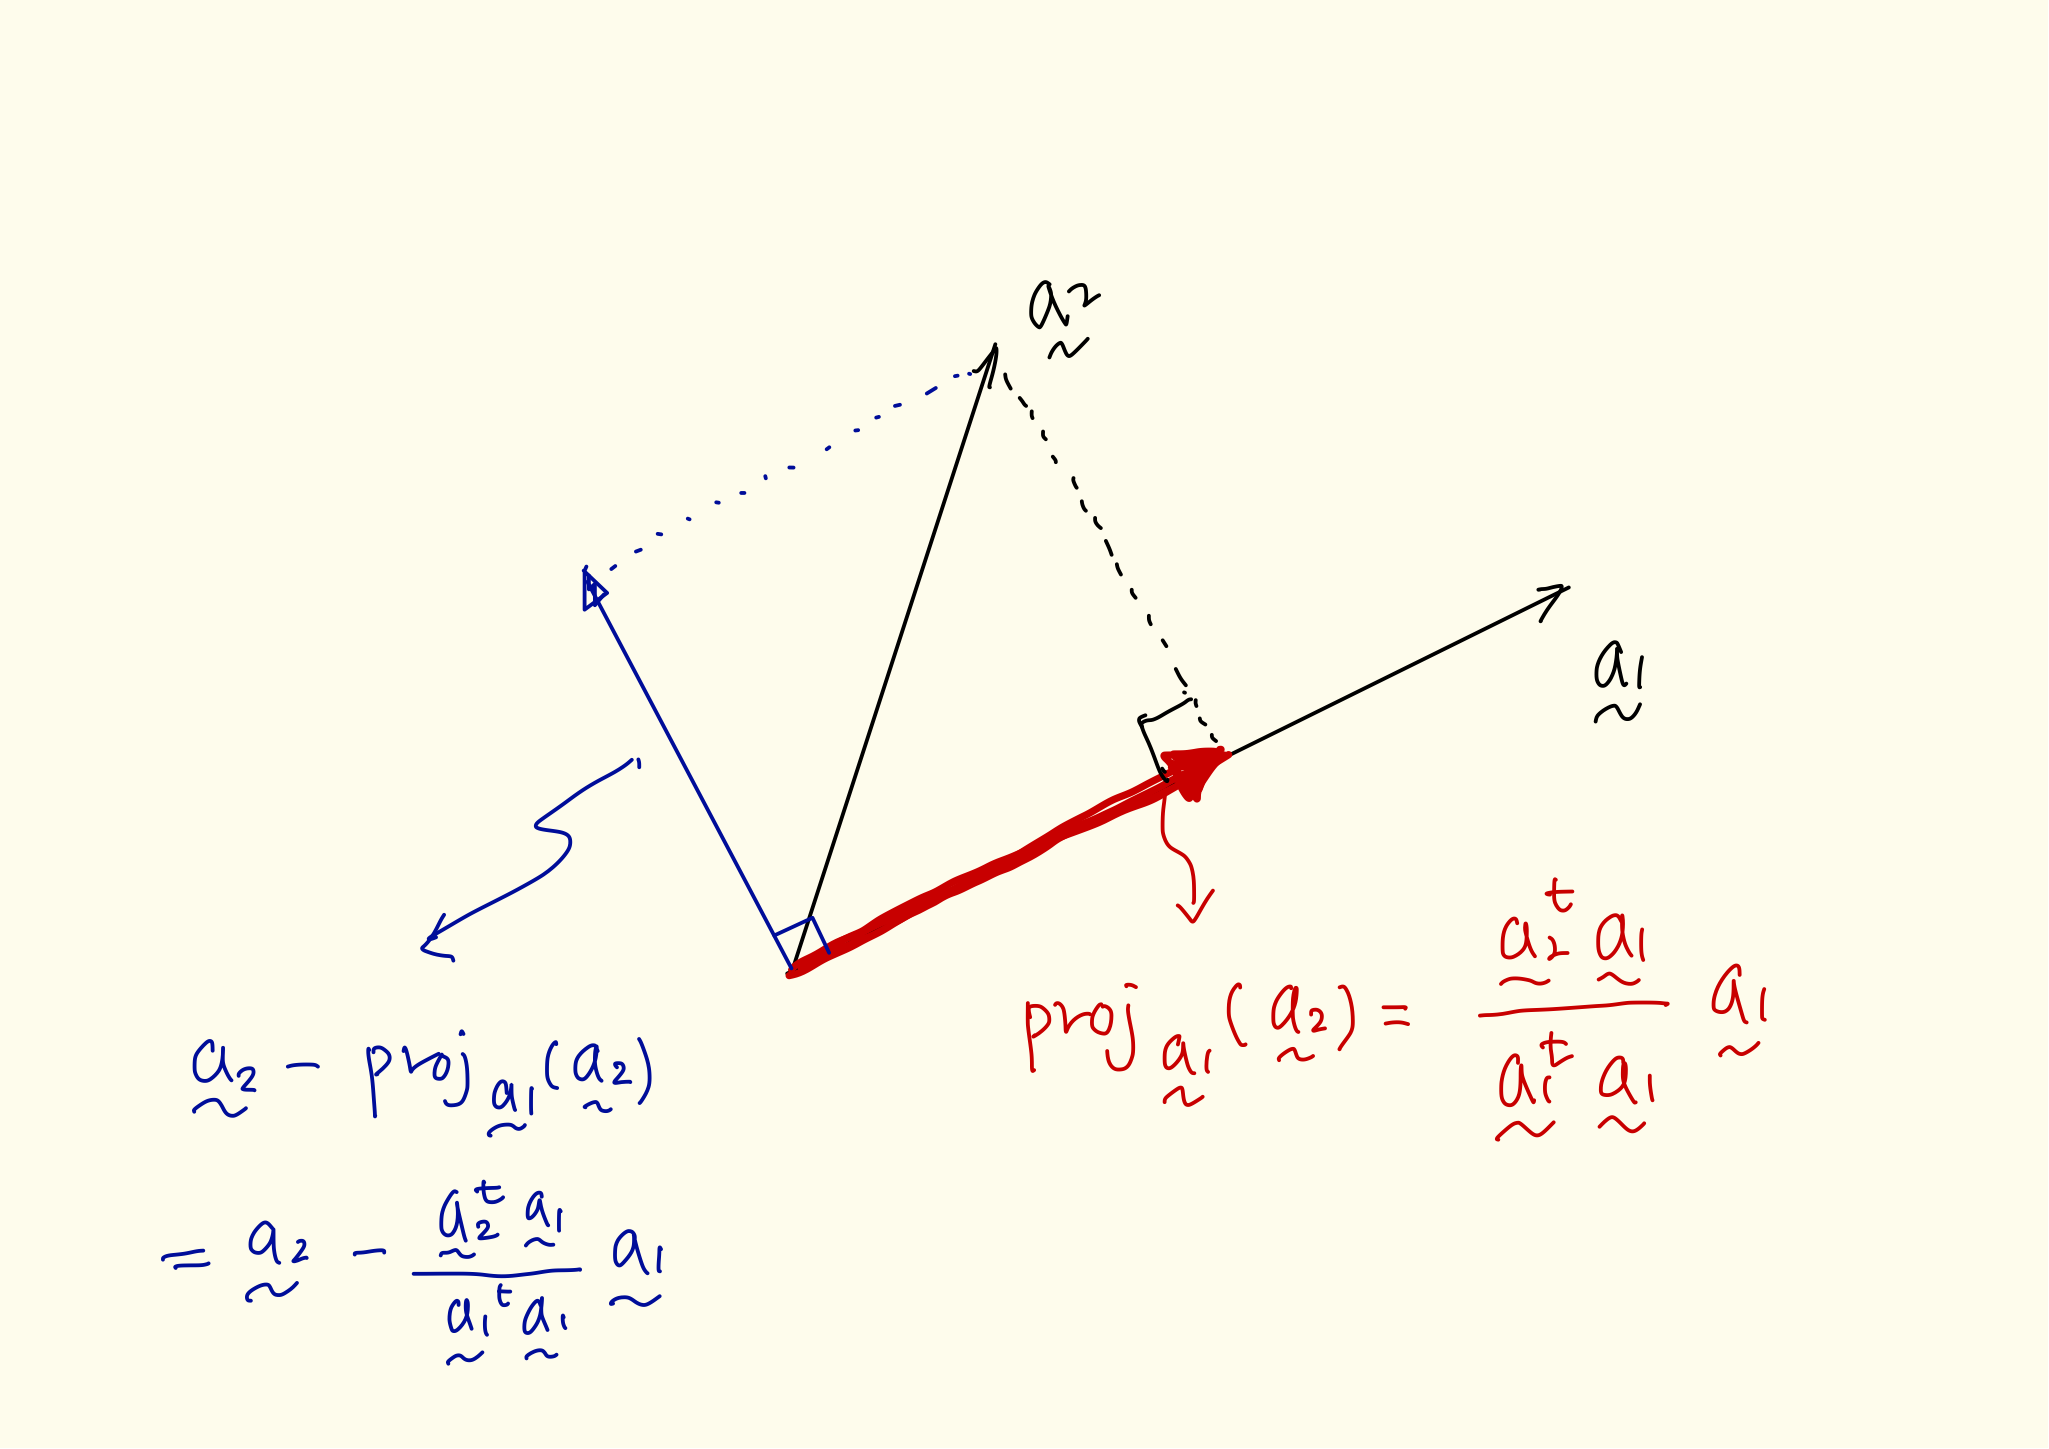
\includegraphics{proj1.png}
\caption{벡터의 사영}
\end{figure}

두 벡터 \(\bm a_1\)와 \(\tilde {\bm q}_2\)의 직교성은 다음과 같이 보일 수 있다.

\begin{align}
\bm a_1^t  \tilde {\bm q}_2 & =
 \bm a_1^t  \left ( \bm a_2 -  \frac{ \bm a_2^t \bm a_1} {\bm a_1^t \bm a_1} \bm a_1 \right ) \notag \\
 & = \bm a_1^t \bm a_2 - \frac{ \bm a_2^t \bm a_1} {\bm a_1^t \bm a_1}  \bm a_1^t \bm a_1 \notag \\
 & = \bm a_1^t \bm a_2 - \bm a_2^t \bm a_1 \notag \\
 & = 0 
 \label{eq:proofortho}
\end{align}

이제 두 벡터 \(\bm q_1\)과 \(\bm q_2\) 를 다음과 같이 정규직교벡터로 만들 수 있다.
\begin{align*}
\bm q_1 & =  \bm a_1 / \norm{\bm a_1 } \\
\bm q_2 & =  \tilde {\bm q}_2 / \norm{\tilde {\bm q}_2}
\end{align*}

\hypertarget{uxcd5cuxc18cuxc81cuxacf1uxbc95uxacfc-uxc0acuxc601}{%
\subsection{최소제곱법과 사영}\label{uxcd5cuxc18cuxc81cuxacf1uxbc95uxacfc-uxc0acuxc601}}

회귀계수벡터의 값을 구하는 최소제곱법의 기준을 다시 살펴보자.

\[   \min_{\bm \beta } \norm{\bm y -  \bm X \bm \beta }^2= \min_{\bm \beta } ( \bm y -  \bm X \bm \beta )^t( \bm y -  \bm X \bm \beta )  \]

위에서 \(\bm X \bm \beta\)는 행렬 \(\bm X\)의 열벡터 \(\bm x_0, \bm x_1, \dots, \bm x_p\) 로 이루어진 선형조합이다.

\[ \bm X \bm \beta = [\bm x_0~\bm x_1~ \cdots \bm x_p]\bm \beta
 = \beta_0 \bm x_0  + \beta_1 \bm x_1 + \cdots + \beta_p \bm x_p \]

따라서 최소제곱법으로 구한 회귀계수 벡터 \(\hat {\bm \beta}\)는 반응값 벡터 \(\bm y\) 와 \(\bm X {\bm \beta}\)의 거리가 최소가 되도록 만들어 준다.

\[ \hat {\bm \beta} = (\bm X^t \bm X)^{-1} \bm X^t \bm y, \quad 
 \min_{\bm \beta } \norm{\bm y -  \bm X \bm \beta }^2 = \norm{\bm y -  \bm X \hat {\bm \beta} }^2
 \]

따라서 예측값 벡터 \(\hat {\bm y}\) 는 행렬 \(\bm X\)의 열벡터로 생성한 열공간 방향으로 반응값 벡터 \(\bm y\)를 사영한 벡터이다.

\[ \hat {\bm y} = \bm X \hat {\bm \beta} = \bm  X(\bm X^t \bm X)^{-1} \bm X^t \bm y \]

위에서 행렬 \(\bm P = \bm X(\bm X^t \bm X)^{-1} \bm X^t\)를 열공간 \(C(\bm X)\)의 사영행렬(projection matrix)라고 부른다.

\begin{figure}
\centering
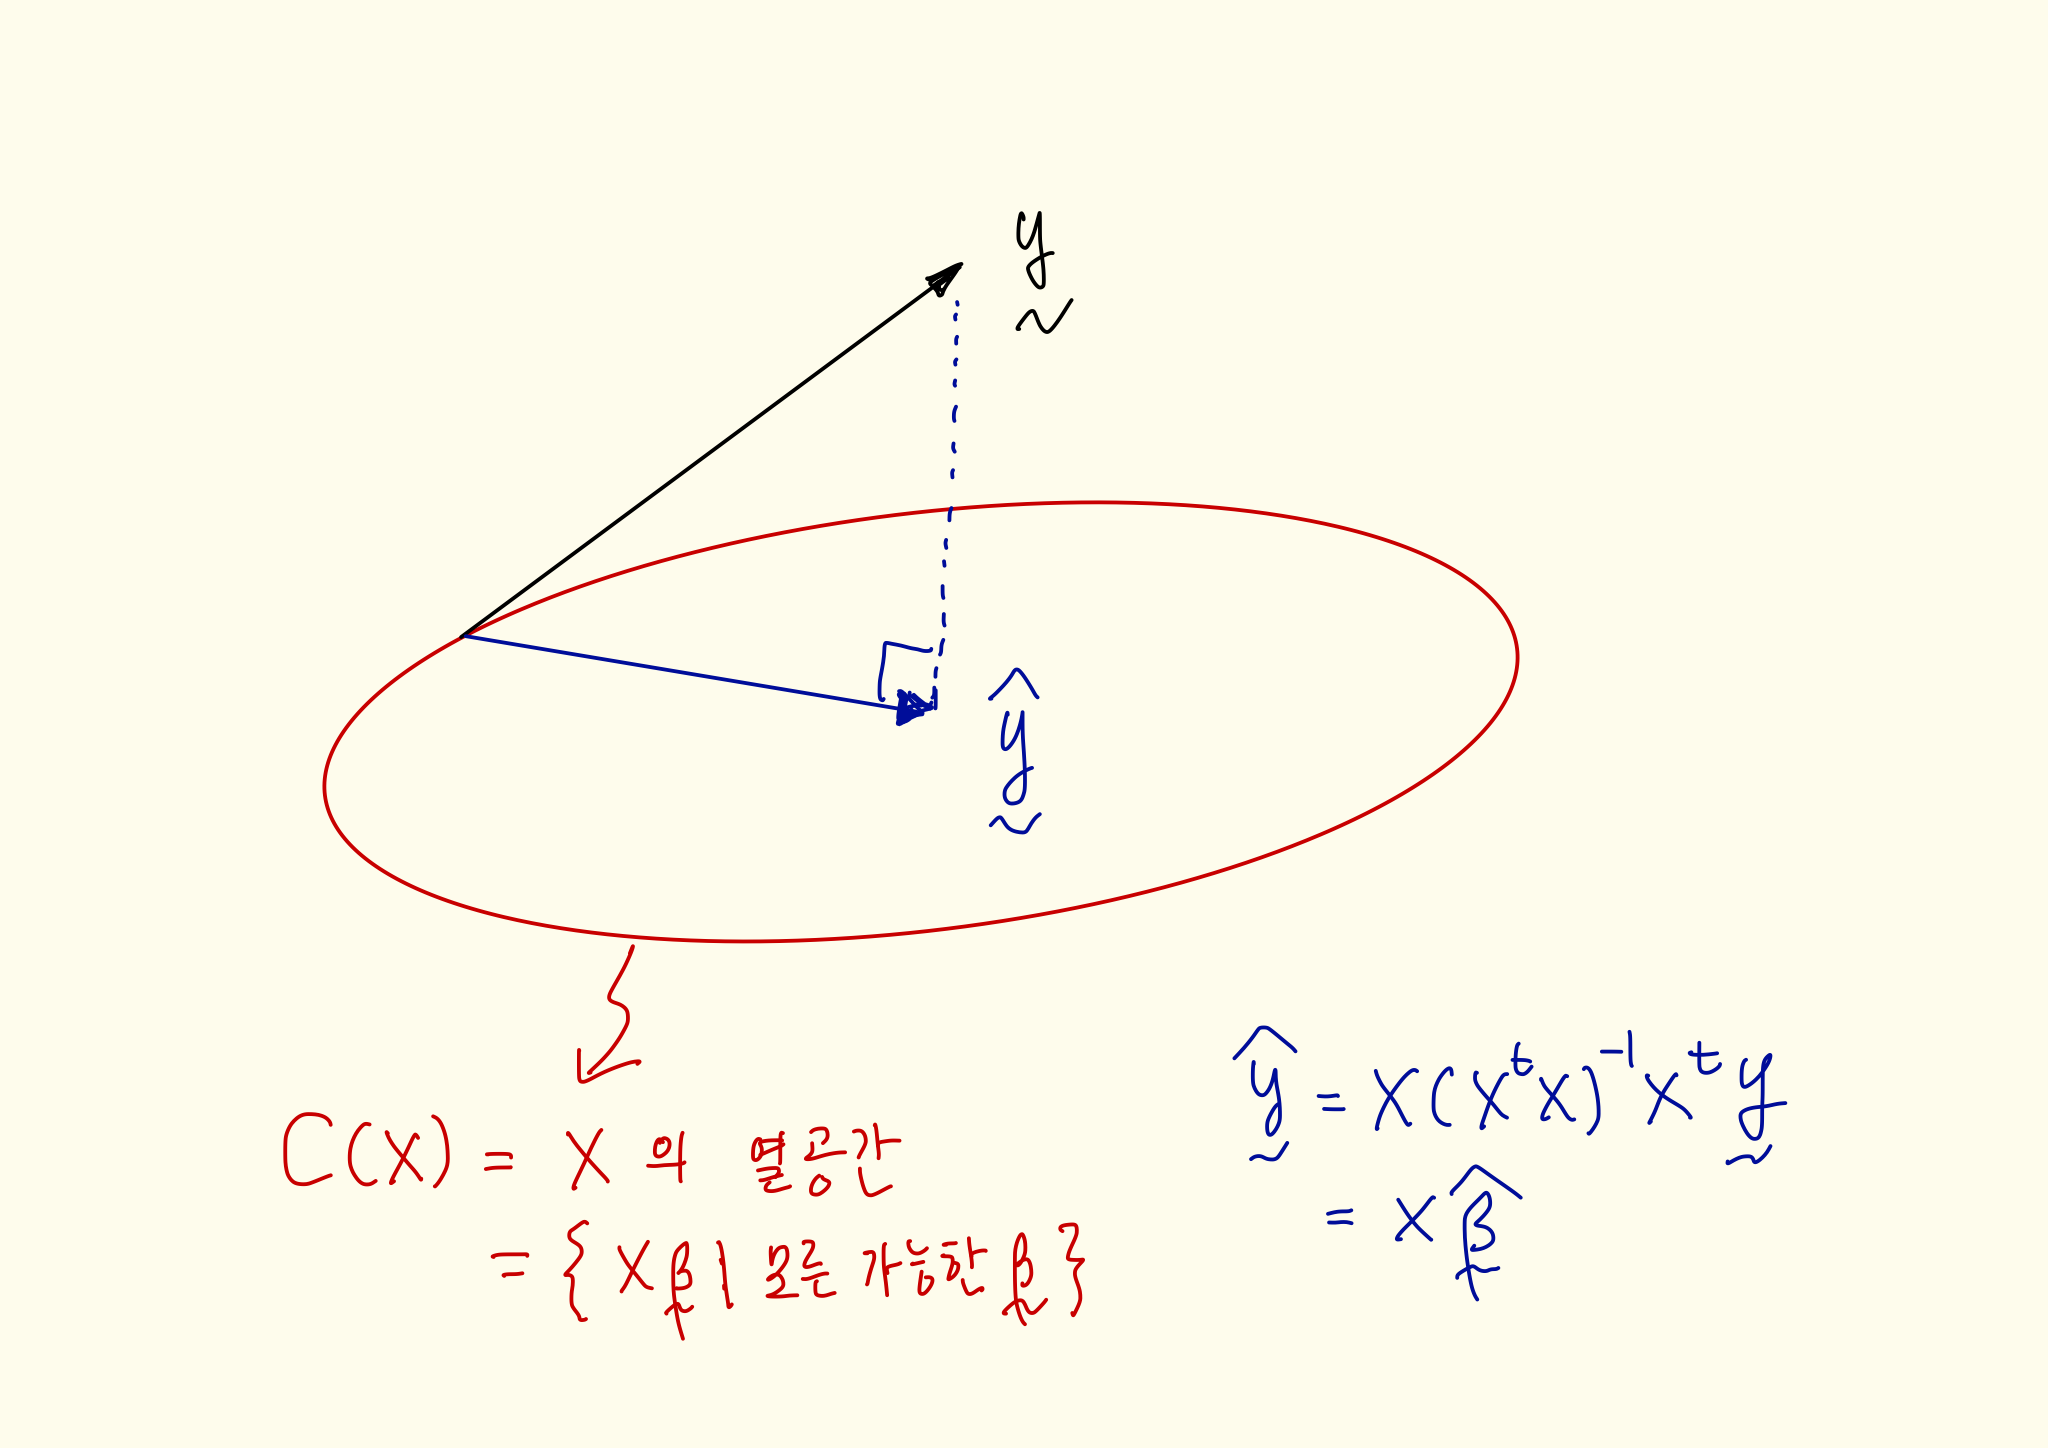
\includegraphics{proj2.png}
\caption{최소제곱법을 설명한 그림}
\end{figure}

\hypertarget{mulivar}{%
\chapter{다변량 확률변수의 성질}\label{mulivar}}

\hypertarget{uxc77cuxbcc0uxb7c9uxbd84uxd3ec}{%
\section{일변량분포}\label{uxc77cuxbcc0uxb7c9uxbd84uxd3ec}}

일변량 확률변수 \(X\)가 확률밀도함수 \(f(x)\)를 가지는 분포를 따를때 기대값과 분산은 다음과 같이 정의된다.
\[ E(X) = \int x f(x)  dx = \mu, \quad V(X) = E[ X-E(X)]^2=\int (x-\mu)^2 f(x) dx =\sigma^2 \]

새로운 확률변수 \(Y\)가 확률변수 \(X\)의 선형변환으로 표시된다면 (\(a\)와 \(b\)는 실수)
\[ Y = aX+b\]
그 기대값(평균)과 분산은 다음과 같이 계산된다.
\begin{eqnarray*}
E(Y) &=& E(aX+b) \\
&=& \int (ax+b) f(x) dx \\
&=& a \int x f(x) dx + b \\
&=& a E(X) + b\\
&=& a \mu + b \\
V(Y) &=& Var(aX+b) \\
&=& E[aX+b -E(aX+b)]^2 \\
&=& E[a(X-\mu)]^2 \\
&=& a^2 E(X-\mu)^2\\
&=& a^2 \sigma^2
\end{eqnarray*}

\hypertarget{uxd655uxb960uxbca1uxd130uxc640-uxbd84uxd3ec}{%
\section{확률벡터와 분포}\label{uxd655uxb960uxbca1uxd130uxc640-uxbd84uxd3ec}}

확률벡터 \(\bm X\)가 \(p\) 차원의 다변량분포를 따른다고 하고 결합확률밀도함수 \(f(\bm x) =f(x_1,x_2,\dots,x_p)\)를
를 가진다고 하자.
\begin{equation*}
\bm X =
  \begin{pmatrix}
X_1 \\
X_2 \\
X_3 \\
..  \\
X_p
\end{pmatrix}
\end{equation*}

다변량 확률벡터의 기대값(평균벡터)과 공분산(행렬)은 다음과 같이 계산된다.
\begin{equation*}
\bm E(\bm X) =
  \begin{pmatrix}
E(X_1) \\
E(X_2) \\
E(X_3) \\
..  \\
E(X_p)
\end{pmatrix}
= 
  \begin{pmatrix}
\mu_1 \\
\mu_2 \\
..  \\
\mu_p
\end{pmatrix}
=\bm \mu
\end{equation*}

\begin{equation*}
V(\bm X) =Cov(\bm X) = E (\bm X-\bm \mu) (\bm X-\bm \mu)^t 
= 
  \begin{pmatrix}
\sigma_{11} & \sigma_{12} & \dots & \sigma_{1p} \\
\sigma_{12} & \sigma_{22} & \dots & \sigma_{2p} \\
& \dots & \dots & \\
\sigma_{1p} & \sigma_{2p} & \dots & \sigma_{pp} \\
\end{pmatrix}
= \bm \Sigma
\end{equation*}
여기서 \(\sigma_{ii}=V(X_i)\), \(\sigma_{ij} = Cov(X_i, X_j)=Cov(X_j, X_i)\)이다. 따라서 공분산 행렬
\(\bm \Sigma\)는 대칭행렬(symmetric matrix)이다. 다음 공식은 유용한 공식이다.
\[ \bm \Sigma = E (\bm X-\bm \mu) (\bm X-\bm \mu)^t  = E(\bm X \bm X^t)-\bm \mu \bm \mu^t \]

두 확률변수의 상관계수 \(\rho_{ij}\)는 다음과 같이 정의된다.
\[ \rho_{ij} = \frac{Cov(X_i, X_j)}{ \sqrt{V(X_i) V(X_j)}} = \frac{\sigma_{ij}}{\sqrt{\sigma_{ii}
  \sigma_{jj}}} \]

새로운 확률벡터 \(\bm Y\)가 확률벡터 \(\bm X\) 의 선형변환라고 하자.
\[ \bm Y = \bm A  \bm X + \bm b \]
단 여기서 \(\bm A = \{ a_{ij} \}\)는 \(p \times p\) 실수 행렬이고
\(\bm b =(b_1 b_2 \dots b_p)^t\)는 \(p \times 1\) 실수 벡터이다.

확률벡터 \(\bm Y\)의 기대값(평균벡터)과 공분산은 다음과 같이 계산된다.
\begin{eqnarray*}
E(\bm Y ) &=& E(\bm A \bm X+ \bm b) \\
&=& \bm A E(\bm X)+ \bm b \\
&=& \bm A \bm \mu+ \bm b \\
V(\bm Y) &=& Var(\bm A \bm X+ \bm b) \\
&=& E[\bm A \bm X+ \bm b -E(\bm A \bm X+ \bm b)] [\bm A \bm X+ \bm b -E(\bm A \bm X+ \bm b)]^t \\
&=& E[\bm A \bm X -  \bm A \bm \mu] [\bm A \bm X -  \bm A \bm \mu]^t \\
&=& E[\bm A (\bm X - \bm \mu)] [\bm A (\bm X - \bm \mu)]^t \\
&=& \bm A E [(\bm X - \bm \mu) (\bm X - \bm \mu)^t] \bm A^t \\
&=& \bm A \bm \Sigma \bm A^t
\end{eqnarray*}

만약 표본 \(\bm X_i, \bm X_2, \dots, \bm X_n\) 이 독립적으로 평균이 \(\bm \mu\) 이고 공분산이 \(\bm \Sigma\)
인 분포에서 추출되었다면 표본의 평균벡터 \(\bar {\bm X}\) 는 평균이 \(\bm \mu\) 이고 공분산이 \(\frac{1}{n}\bm \Sigma\)
인 분포를 따른다.
\begin{equation*}
\bar {\bm X} =
  \begin{pmatrix}
\sum_{i=1}^n X_{i1} / n  \\
\sum_{i=1}^n X_{i2} / n \\
\sum_{i=1}^n X_{i3} / n \\
..  \\
\sum_{i=1}^n X_{ip} / n 
\end{pmatrix}
\end{equation*}
여기서 \(X_{ij}\) 는 \(i\)번째 표본벡터 \(\bm X_i =(X_{i1} X_{i2} \dots X_{ip})^t\)의 \(j\)번째 확률변수이다.

\hypertarget{uxb2e4uxbcc0uxb7c9-uxc815uxaddcuxbd84uxd3ec}{%
\section{다변량 정규분포}\label{uxb2e4uxbcc0uxb7c9-uxc815uxaddcuxbd84uxd3ec}}

일변량 확률변수 \(X\)가 평균이 \(\mu\) 이고 분산이 \(\sigma^2\)인 정규분포를 따른다면 다음과 같이 나타내고 \[ X \sim N(\mu, \sigma^2 ) \]
확률밀도함수 \(f(x)\) 는 다음과 갇이 주어진다.
\[ f(x) = (2 \pi \sigma^2)^{-1/2} \exp \left ( - \frac{(x-\mu)^2}{2} \right ) \]

\(p\)-차원 확률벡터 \(\bm X\)가 평균이 \(\bm \mu\) 이고 공분산이 \(\bm \Sigma\)인
다변량 정규분포를 따른다면 다음과 같이 나타내고 \[ \bm X \sim N_p(\bm \mu, \bm \Sigma ) \]
확률밀도함수 \(f(\bm x)\) 는 다음과 갇이 주어진다.
\[ f(\bm x) = (2 \pi)^{-p/2} | \bm \Sigma|^{-1/2} 
   \exp \left ( - \frac{(\bm x-\bm \mu) \bm \Sigma^{-1}(\bm x-\bm \mu)^t}{2} \right ) \]

다변량 정규분포 \(N(\bm \mu, \bm \Sigma)\)를 따르는 확률벡터 \(\bm X\)를 다음과 같이 두 부분으로 나누면

\[ 
  \bm X = 
    \begin{bmatrix}
  \bm X_1 \\
  \bm X_2
  \end{bmatrix}, \quad
  \bm X_1 = 
    \begin{bmatrix}
  \bm X_{11} \\
  \bm X_{12} \\
  \bm \vdots \\
  \bm X_{1p}
  \end{bmatrix}, \quad 
  \bm X_2= 
    \begin{bmatrix}
  \bm X_{21} \\
  \bm X_{22} \\
  \bm \vdots \\
  \bm X_{2q}
  \end{bmatrix}
  \]

각각 다변량 정규분포를 따르고 다음과 같이 나타낼 수 있다.

\[ 
  \begin{bmatrix}
  E(\bm X_1) \\
  E(\bm X_2)
  \end{bmatrix}
  =
    \begin{bmatrix}
  \bm \mu_1 \\
  \bm \mu_2
  \end{bmatrix}
  , \quad 
  \begin{bmatrix}
  V(\bm X_1) & Cov(\bm X_1, X_2) \\
  Cov(\bm X_2 X_1) & V(\bm X_2)
  \end{bmatrix}
  =
    \begin{bmatrix}
  \bm \Sigma_{11} & \bm \Sigma_{12} \\
  \bm \Sigma^t_{12} & \bm \Sigma_{22}
  \end{bmatrix}
  \]

\[  \bm X =
    \begin{bmatrix}
  \bm X_1 \\
  \bm X_2
  \end{bmatrix}
  \sim
  N_{p+q} \left (
    \begin{bmatrix}
    \bm \mu_1 \\
    \bm \mu_2
    \end{bmatrix}
    ,\begin{bmatrix}
    \bm \Sigma_{11} & \Sigma_{12} \\
    \bm \Sigma^t_{12} & \Sigma_{22}
    \end{bmatrix}
    \right )
  \]

확률벡터 \(\bm X_2 = \bm x_2\)가 주어진 경우 \(\bm X_1\)의 조건부 분포는 \(p\)-차원 다변량 정규분포를 따르고 평균과 공분산은 다음과 같다.

\[ 
  E(\bm X_1 | \bm X_2 = \bm x_2 ) = \bm \mu_1 + \bm \Sigma_{12} \bm \Sigma^{-1}_{22} (\bm \mu_2 - \bm x_2), \quad
  V(\bm X_1 | \bm X_2 = \bm x_2 )  = \bm \Sigma_{11} -\bm \Sigma_{12} \bm \Sigma^{-1}_{22} \bm \Sigma^t_{12}
  \]

예를 들어 \(2\)-차원 확률벡터 \(\bm X=(X_1, X_2)^t\)가 평균이 \(\bm \mu=(\mu_1,\mu_2)^t\) 이고
공분산 \(\bm \Sigma\)가 다음과 같이 주어진
\begin{equation*}
\bm \Sigma =
  \begin{pmatrix}
\sigma_{11} & \sigma_{12} \\
\sigma_{12} & \sigma_{22}
\end{pmatrix}
\end{equation*}
이변량 정규분포를 따른다면 확률밀도함수 \(f(\bm x)\)에서 \(\exp\)함수의 인자는 다음과 같이 주어진다.
\begin{eqnarray*}
&(\bm x-\bm \mu) \bm \Sigma^{-1}(\bm x-\bm \mu)^t
= \\
&-\frac{1}{2 (1-\rho^2)} 
\left [ 
  \left ( \frac{(x_1-\mu_1)^2}{\sigma_{11}} \right )
  +\left ( \frac{(x_2-\mu_2)^2}{\sigma_{22}} \right )
  -2 \rho \left ( \frac{(x_1-\mu_1)}{\sqrt{\sigma_{11}}} \right )
  \left ( \frac{(x_2-\mu_2)}{\sqrt{\sigma_{22}}} \right )
  \right ]
\end{eqnarray*}
그리고 \(p=2\)인 경우 확률밀도함수의 상수부분은 다음과 같이 주어진다.
\[ (2 \pi)^{-p/2} | \bm \Sigma|^{-1/2} = \frac{1}{ 2 \pi \sqrt{\sigma_{11} \sigma_{22} (1-\rho^2)}} \]
여기서 \(\rho = \sigma_{12} / \sqrt{\sigma_{11} \sigma_{22}}\)

만약 \(X_2 = x_2\)가 주어졌을 때 \(X_1\)의 조건부 분포는 정규분포이고 평균과 분산은 다음과 같이 주어진다.

\[ 
  E( X_1 |  X_2 =  x_2 ) =  \mu_1 +  \frac{\sigma_{12}}{\sigma_{22}} ( \mu_2 -  x_2)  = \mu_1 +  \rho \frac{\sqrt{\sigma_{11}}}{\sqrt{\sigma_{22}}} ( \mu_2 -  x_2) \]

\[
  V( X_1 |  X_2 =  x_2 )  =  \sigma_{11} - \frac{\sigma^2_{12}}{\sigma_{22}}  = \sigma_{11}(1-\rho^2)
  \]

다변량 정규분포에서 공분산이 0인 두 확률 변수는 독립이다.
\[ \sigma_{ij} = 0 \leftrightarrow X_i \text{ and } X_j \text{ are independent} \]

\hypertarget{uxd45cuxc900uxc815uxaddcuxbd84uxd3ecuxb85cuxc758-uxbcc0uxd658}{%
\section{표준정규분포로의 변환}\label{uxd45cuxc900uxc815uxaddcuxbd84uxd3ecuxb85cuxc758-uxbcc0uxd658}}

일변량 확률변수 \(X\)가 평균이 \(\mu\) 이고 분산이 \(\sigma^2\)인 경우 다음과 같은 선형변환을 고려하면.
\[ Z = \frac{X - \mu}{\sigma} = (\sigma^2)^{-1/2} (X-\mu) \]
확률변수 \(Z\) 는 평균이 \(0\) 이고 분산이 \(1\)인 분포를 따른다.

\(p\)차원 확률벡터 \(\bm X\) 가 평균이 \(\bm \mu\) 이고 공분산이 \(\bm \Sigma\)인 분포를 가진다고 가정하자.
공분산 행렬 \(\bm \Sigma\)는 양정치 행렬(positive definite matrix)이며 다음과 같은 행렬의 분해가 가능하다.
\[ \Sigma = \bm C \bm C^t \]
여기서 \(\bm C\) 는 정칙행렬이며 역행렬 \(\bm C^{-1}\)가 존재한다.
위와 같은 행렬의 분해는 스펙트럴 분해(spectral decomposition)을 이용하여 구할 수 있다. 공분산 행렬 \(\bm \Sigma\)는 양정치 행렬이므로 고유치(eigen value) \((\lambda_1, \lambda_2,\dots, \lambda_p)\)가 모두 양수이고 정규직교 고유벡터(orthonormal eigen vector)의 행렬 \(\bm P\)을 이용하여 다음과 같은 분해가 가능하다.
\[ \Sigma = \bm P \bm \Lambda \bm P^t = \bm P \bm \Lambda^{1/2} \Lambda^{1/2} \bm P^t \]
여기서 \(\bm \Lambda\)는 고유치 \((\lambda_1, \lambda_2,\dots, \lambda_p)\)를 대각원소로 가지는
대각행렬이며 \(\bm \Lambda^{1/2}\)는 고유치의 제곱근을 대각원소로 가지는
대각행렬이다. 따라서 \(\bm C = \bm P \bm \Lambda^{1/2}\)로 하면 위와 같은 행렬의 분해가 가능하다.
정규직교 고유벡터(orthonormal eigen vector)의 행렬 \(\bm P\)는 직교행렬이므로
\[ \bm C^{-1} =  (\bm P \bm \Lambda^{1/2})^{-1} = \bm \Lambda^{-1/2} \bm P^t \]

\(p\)차원 확률벡터 \(\bm X\)의 다음과 같은 선형변환을 고려하면.
\[ \bm Z = \bm C^{-1} ( \bm X- \bm \mu) = \bm \Lambda^{-1/2} \bm P^t ( \bm X- \bm \mu)  \]
확률벡터 \(\bm Z\) 는 평균이 \(\bm 0\) 이고 공분산이 \(\bm I\)인 분포를 따른다 (why?).

확률벡터 \(\bm X\)가 정규분포를 따른다면 선형변환한 확률벡터 \(\bm Z\)도 정규분포를 따른다.

\hypertarget{uxc608uxc81c}{%
\section{예제}\label{uxc608uxc81c}}

예를 들어 이변량확률벡터 \(\bm X\)가 다음과 같은 평균벡터와 공분산을 가진 정규분포를 따른다고 하자
\begin{equation*}
\bm \mu =
  \begin{pmatrix}
1\\
2
\end{pmatrix}
\quad
\bm \Sigma =
  \begin{pmatrix}
2 & 1\\
1 & 2
\end{pmatrix}
\end{equation*}

공분산행렬 \(\bm \sigma\)의 고유치는 \(|\bm \sigma -\lambda \bm I|=0\)의 방정식을 풀어 구할 수 있다.
\begin{equation*}
|\bm \sigma -\lambda \bm I|  =
  \begin{pmatrix}
2-\lambda & 1\\
1 & 2-\lambda
\end{pmatrix}
= \lambda^2 -4 \lambda +3=0
\end{equation*}
방정식을 풀면 고유치는 \((\lambda_1, \lambda_2) = (3,1)\)이다. 각 고유치에 대한 고유벡터 \(\bm p=(p_1, p_2)^t\)는 \(\bm \Sigma \bm p = \lambda \bm p\) 으로 구할 수 있다. 각 고유치에 대하여 방정식을 구하면 다음 두 개의 방정식을 얻을 수 있다.
\begin{equation*}
p_1 - p_2 = 1 \text{ and } p_1 + p_2 = 0
\end{equation*}
정규직교 벡터의 조건을 만족 시키기 위해서 \(p^2_1 + p^2_2=1\)의 조건을 적용하면 다음과 같은
정규직교 고유행렬을 얻을 수 있다.
\begin{equation*}
\bm P =
  \begin{pmatrix}
\frac{1}{\sqrt{2}} & -\frac{1}{\sqrt{2}}\\
\frac{1}{\sqrt{2}} & \frac{1}{\sqrt{2}}
\end{pmatrix}
\end{equation*}
또한
\begin{equation*}
\bm \Lambda =
  \begin{pmatrix}
3 & 0\\
0 & 1
\end{pmatrix}
\quad
\bm \Lambda^{1/2} =
  \begin{pmatrix}
\sqrt{3} & 0\\
0 & 1
\end{pmatrix}
\end{equation*}
따라서 \(C^{-1} = \Lambda^{-1/2} \bm P^t\) 이며
\begin{equation*}
\bm C^{-1} =
  \bm \Lambda^{-1/2} \bm P^t =
  \begin{pmatrix}
\frac{1}{\sqrt{3}} & 0\\
0 & 1
\end{pmatrix}
\begin{pmatrix}
\frac{1}{\sqrt{2}} & \frac{1}{\sqrt{2}}\\
-\frac{1}{\sqrt{2}} & \frac{1}{\sqrt{2}}
\end{pmatrix}
=
  \begin{pmatrix}
\frac{1}{\sqrt{6}} & \frac{1}{\sqrt{6}}\\
-\frac{1}{\sqrt{2}} & \frac{1}{\sqrt{2}}
\end{pmatrix}
\end{equation*}

위의 계산을 R 프로그램으로 다음과 같이 구현할 수 있다.

\begin{Shaded}
\begin{Highlighting}[]
\NormalTok{mu }\OtherTok{\textless{}{-}} \FunctionTok{c}\NormalTok{(}\DecValTok{1}\NormalTok{,}\DecValTok{2}\NormalTok{)}
\NormalTok{S }\OtherTok{\textless{}{-}} \FunctionTok{matrix}\NormalTok{(}\FunctionTok{c}\NormalTok{(}\DecValTok{2}\NormalTok{,}\DecValTok{1}\NormalTok{,}\DecValTok{1}\NormalTok{,}\DecValTok{2}\NormalTok{),}\DecValTok{2}\NormalTok{,}\DecValTok{2}\NormalTok{)}
\NormalTok{res}\OtherTok{\textless{}{-}} \FunctionTok{eigen}\NormalTok{(S)}
\NormalTok{res}
\end{Highlighting}
\end{Shaded}

\begin{verbatim}
## eigen() decomposition
## $values
## [1] 3 1
## 
## $vectors
##           [,1]       [,2]
## [1,] 0.7071068 -0.7071068
## [2,] 0.7071068  0.7071068
\end{verbatim}

\begin{Shaded}
\begin{Highlighting}[]
\NormalTok{L }\OtherTok{\textless{}{-}}\NormalTok{ res}\SpecialCharTok{$}\NormalTok{values}
\NormalTok{P }\OtherTok{\textless{}{-}}\NormalTok{ res}\SpecialCharTok{$}\NormalTok{vectors}
\NormalTok{Lsqrt }\OtherTok{\textless{}{-}} \FunctionTok{diag}\NormalTok{(}\FunctionTok{sqrt}\NormalTok{(L))}
\NormalTok{C }\OtherTok{\textless{}{-}}\NormalTok{ P }\SpecialCharTok{\%*\%}\NormalTok{ Lsqrt}
\NormalTok{C}
\end{Highlighting}
\end{Shaded}

\begin{verbatim}
##          [,1]       [,2]
## [1,] 1.224745 -0.7071068
## [2,] 1.224745  0.7071068
\end{verbatim}

\begin{Shaded}
\begin{Highlighting}[]
\NormalTok{Cinv }\OtherTok{\textless{}{-}} \FunctionTok{solve}\NormalTok{(C)}
\NormalTok{Cinv }
\end{Highlighting}
\end{Shaded}

\begin{verbatim}
##            [,1]      [,2]
## [1,]  0.4082483 0.4082483
## [2,] -0.7071068 0.7071068
\end{verbatim}

\begin{Shaded}
\begin{Highlighting}[]
\NormalTok{Cinv }\SpecialCharTok{\%*\%}\NormalTok{ S }\SpecialCharTok{\%*\%} \FunctionTok{t}\NormalTok{(Cinv)}
\end{Highlighting}
\end{Shaded}

\begin{verbatim}
##      [,1] [,2]
## [1,]    1    0
## [2,]    0    1
\end{verbatim}

\hypertarget{quadratic}{%
\chapter{이차형식의 분포}\label{quadratic}}

\hypertarget{uxbe44uxc911uxc2ec-chi2-uxbd84uxd3ec}{%
\section{\texorpdfstring{비중심 \(\chi^2\) 분포}{비중심 \textbackslash chi\^{}2 분포}}\label{uxbe44uxc911uxc2ec-chi2-uxbd84uxd3ec}}

만약 확률변수 \(x\)가 \(N(\mu, 1)\)을 따른다면 \(v=x^2\)은 비중심 \(\chi^2\) 분포, \(\chi^2_1(\lambda^2)\) 를 따른다. 여기서 비중심 \(\chi^2\) 분포의 자유도는 1이고 비중심모수 \(\lambda^2 = \mu^2\)으로 주어진다.

만약 확률변수 \(x\)가 \(N(0, 1)\)을 따른다면 \(v=x^2\)은 중심 \(\chi^2\) 분포, \(\chi^2_1\) 를 따르며 이때는 비중심모수가 \(\lambda^2=0\)이다.

이제 \(n\)개의 서로 독립인 확률 변수 \(x_1,x_2,\cdots,x_n\)이 각각 \(N(\mu_i, 1)\)을 따른다면 \(v=x_1^2+\dots+x_n^2\)은 자유도가 \(n\)이고 비중심 모수가 \(\lambda^2 = \sum_{i=1}^n \mu_i^2\)인 비중심 \(\chi^2\) 분포, \(\chi^2_n(\lambda^2)\) 를 따른다. 비중심모수가 0 이면 자유도가 \(n\)인 (중심) 카이제곱 분포를 따른다.

\hypertarget{uxc774uxcc28uxd615uxc2dduxc758-uxbd84uxd3ec}{%
\section{이차형식의 분포}\label{uxc774uxcc28uxd615uxc2dduxc758-uxbd84uxd3ec}}

\(n\)개의 서로 독립인 확률 변수 \(x_1,x_2,\cdots,x_n\)이 각각 \(N(\mu_i, \sigma^2)\)를 따른다면
\(n\)-차원의 확률벡터 \(\bm x\)는 다음과 같은 다변량 정규분포를 따른다고 할 수 있다.

\[ \bm x \sim N(\bm \mu, \sigma^2 \bm I) \]

위에서 \(\bm \mu^t =(\mu_1, \mu_2, \dots, \mu_n)\)

이제 이차형식의 분포에 대하여 논의하자.

\begin{theorem}[Distribution of quadratic form]
\protect\hypertarget{thm:unnamed-chunk-16}{}{\label{thm:unnamed-chunk-16} \iffalse (Distribution of quadratic form) \fi{} }\(n\)-차원의 확률벡터 \(\bm x\)가 \(N(\bm \mu, \sigma^2 \bm I)\)를 따른 다면 이차형식 \(Q=\bm x^t \bm A \bm x\)의 분포는 다음과 같다.

\begin{equation}
V = \frac{Q}{\sigma^2} = \frac {\bm x^t \bm A \bm x}{\sigma^2} ~~ \equiv_d ~~ \sum_{i=1}^n \lambda_i \frac{u^2_i}{\sigma^2}
\label{eq:quaddist1}
\end{equation}

위에서 행렬 \(\bm A\)의 스펙트럴 분해는 \(\bm A = \bm P \bm \Lambda \bm P^t\)이며 \(\lambda_i\)는 행렬 \(\bm A\)의 고유치, 즉 행렬 \(\bm \Lambda\)의 대각원소이다. 또한 확률변수 \(u_i\)들은 서로 독립이며 정규분포 \(N(\eta_i, \sigma^2)\)를 따른다. 여기서 \(\eta_1, \eta_2,\dots, \eta_n\)는 다음과 같이 정의된다.
\[ 
\bm \eta =
\begin{bmatrix}
\eta_1 \\
\eta_2 \\
\vdots \\
\eta_n 
\end{bmatrix} =
  \bm P^t \bm \mu
\]
즉, 식 \eqref{eq:quaddist1}에서 \(u_1^2/\sigma^2, u_2^2/\sigma^2, \dots, u_n^2/\sigma^2\)는 서로 독립이며 각각 자유도가 1 이고 비중심 모수가 \(\eta_1^2/\sigma^2, \eta_2^2/\sigma^2, \dots, \eta_n^2/\sigma^2\)인 비중심 \(\chi^2\)-분포를 따른다. \(\blacksquare\)
\end{theorem}

위의 정리의 증명은 다음과 같은 변환를 이용한다.

\[ 
\frac{\bm x^t \bm A \bm x}{\sigma^2}  = \frac{\bm x^t \bm P \bm \Lambda \bm P^t \bm x}{\sigma^2}   = \frac{\bm u^t \bm \Lambda  \bm u}{\sigma^2} = \sum_{i=1}^n \lambda_i \left [ \frac{u_i}{\sigma} \right ]^2 
\]

여기서 확률벡터 \(\bm u = \bm P^t \bm x\) 는 \(N(\bm P^t \bm \mu, \sigma^2 \bm P^t \bm P ) = N(\bm \eta, \sigma^2 \bm I)\)를 따른다.

식 \eqref{eq:quaddist1}에서 나타난 이차형식의 분포는 비중심 카이제곱 분포를 따르는 \textbf{서로 독립인인 확률 변수들의 가중 평균}과 같다는 것이다. 이는 이차형식의 분포가 비중심 카이제곱 분포를 따른다는 것이 아님을 주의해야 한다. 그러면 어느 경우에 이차형식의 분포가 비중심 카이제곱 분포를 따르는가 생각해 보자. 가장 쉽게 생각할 수 있는 경우가 식 \eqref{eq:quaddist1}에서 \(\lambda_i\)들의 값들이 0 또는 1인 경우이다. 이러한 경우는 행렬 \(\bm A\)가 멱등행렬인 경우이다. 실제로 다음 정리는 이차형식의 분포가 비중심 카이제곱 분포를 따르는 필요충분 조건이 행렬 \(\bm A\)가 멱등행렬이라는 것을 말해준다.

\begin{corollary}
\protect\hypertarget{cor:unnamed-chunk-17}{}{\label{cor:unnamed-chunk-17} }\(n\)-차원의 확률벡터 \(\bm x\)가 \(N(\bm \mu, \sigma^2 \bm I)\)를 따른다면 이차형식 \(\bm x^t \bm A \bm x /\sigma^2\)의 분포가 자유도가 \(r\)이며 다음과 같은 비중심 모수 \(\lambda^2\)을 가지는 비중심 카이제곱 분포를 따르는 필요충분 조건은 \(\bm A\)가 멱등행렬이고 계수가 \(rank(\bm A =r)\)인 경우이다.

\[ \lambda^2 = \frac{\bm \mu^t \bm A \bm \mu}{\sigma^2} \]

더 나아가 \(\bm A \bm \mu=\bm 0\)인 경우에는 자유도가 \(r\)인 (중심)카이제곱 분포를 따른다. \(\blacksquare\)
\end{corollary}

참고로 이차형식의 기대값과 분산은 다음과 같이 주어진다.

\begin{equation}
E(\bm x^t \bm A \bm x) = \sigma^2 tr(\bm A) + \bm \mu^t \bm A \bm \mu, \quad
V(\bm x^t \bm A \bm x) = 2 \sigma^4 tr(\bm A^2) +4 \sigma^2 \bm \mu^t \bm A^2 \bm \mu
\label{eq:quadmean}
\end{equation}

\hypertarget{uxc774uxcc28uxd615uxc2dduxc758-uxb3c5uxb9bd}{%
\section{이차형식의 독립}\label{uxc774uxcc28uxd615uxc2dduxc758-uxb3c5uxb9bd}}

두 개의 이차형식이 독립일 조건은 다음 정리와 같다.

\begin{theorem}[independence of quadratic forms]
\protect\hypertarget{thm:unnamed-chunk-18}{}{\label{thm:unnamed-chunk-18} \iffalse (independence of quadratic forms) \fi{} }\(n\)-차원의 확률벡터 \(\bm x\)가 \(N(\bm \mu, \sigma^2 \bm I)\)를 따른다고 하자. 두 이차형식 \(Q_1=\bm x^t \bm A \bm x\) 과 \(Q_2=\bm x^t \bm B \bm x\) 가 서로 독립일 필요충분 조건은
\(\bm A \bm B= \bm 0\)이다. \(\blacksquare\)
\end{theorem}

만약 3개의 이차형식 \(Q, Q_1, Q_2\)가 있어서 다음과 같은 관계가 있다고 하자.

\[ Q =\bm x^t \bm A \bm x =  Q_1 + Q_2 =\bm x^t \bm A_1 \bm x + \bm x^t \bm A_2 \bm x \]

이러한 경우 두 이차형식 \(Q\)과 \(Q_1\)이 각각 카이제곱 분포를 따를 때 \(Q_2 = Q-Q_1\)이 카이제곱 분포를 따르는 조건이 중요하다. 다음 정리는 그 조건을 행렬 \(\bm A_2\)가 양반정치인 경우라는 것을 말해준다.

\begin{theorem}
\protect\hypertarget{thm:unnamed-chunk-19}{}{\label{thm:unnamed-chunk-19} }\(n\)-차원의 확률벡터 \(\bm x\)가 \(N(\bm \mu, \sigma^2 \bm I)\)를 따른다고 하자. 세 개의 이차형식 \(Q=\bm x^t \bm A \bm x\), \(Q_1=\bm x^t \bm A_1 \bm x\), \(Q_2=\bm x^t \bm A_2 \bm x\) 가 있다고 하고 \(Q=Q_1+Q_2\)인 관계를 가진다고 가정하자.

만약 \(Q/\sigma^2\)이 \(\chi^2_r(\lambda^2)\)을 따르고 \(Q_1/\sigma^2\)이 \(\chi^2_{r_1}(\lambda_1^2)\)을 따르며 행렬 \(\bm A_2\)가 양반정치 행렬이면 다음을 만족한다.

두 이차형식 \(Q_1\)과 \(Q_2\)는 서로 독립이다. 또한 이차형식 \(Q_2\)는 자유도가 \(r_2 = r-r_1\)이고 비중심 모수가 \(\lambda_2^2 = \lambda^2 -\lambda_1^2\)인 비중신ㅁ 카이제곱분포를 따른다. \(\blacksquare\)
\end{theorem}

\hypertarget{uxcf54uxd06cuxb780uxc758-uxc815uxb9ac}{%
\section{코크란의 정리}\label{uxcf54uxd06cuxb780uxc758-uxc815uxb9ac}}

선형모형에서 자주 등장하는 제곱합들의 분해, 즉 이차형식의 분해를 생각할 때 각 제곱합들의 분포를 아는 것이 매우 중요하다. 다음에 제시된 코크란의 정리(Chchran's Theorem)는 총 제곱합을 분해했을 때 각 제곱합의 분포가 카이제곱 분포를 따를 조건을 말해준다.

\begin{theorem}[COCHRAN'S THEOREM]
\protect\hypertarget{thm:unnamed-chunk-20}{}{\label{thm:unnamed-chunk-20} \iffalse (COCHRAN'S THEOREM) \fi{} }\(n\)-차원의 확률벡터 \(\bm x\)가 \(N(\bm \mu, \sigma^2 \bm I)\)를 따른다고 하자. \(k\) 개의 이차형식 \(Q_j=\bm x^t \bm A_j \bm x\), \(j=1,2,\dots,k\)를 생각하고 다음과 같은 관계를 가진다고 하자.

\[ \bm x^t \bm x = \sum_{i=1}^n x_i^2 = \sum_{j=1}^k Q_j \]

즉, \(\sum_{j=1}^k \bm A_j = \bm I\)이다. 또한 \(r_j =rank(\bm A_j)\) 이고 \(\lambda_j^2 = \bm \mu^t \bm A_{j} \bm \mu\) 라고 하자.

\(k\)개의 이차형식 \(Q_1, Q_2, \dots , Q_k\) 들이 모두 독립이고 각 이차형식 \(Q_j/\sigma^2\)가 비중심 카이제곱 분포 \(\chi^2_{r_{j}}(\lambda_j^2)\)를 따를 필요중분 조건은 다음과 같다.

\begin{equation}
r_1 + r_2 + \dots + r_{k} = n
\label{eq:cochran}
\end{equation}

\(\blacksquare\)
\end{theorem}

이제 제곱합의 분포들에 대하여 지금까지 학습한 내용을 정리해보자. 만약 \(n\)-차원의 확률벡터 \(\bm x\)가 \(N(\bm \mu, \sigma^2 \bm I)\)를 따른다고 하고 위의 코크란의 정리와 같이 제곱합의 분해를 고려하자. 다음에 제시된 모든 문장은 서로 동치(equivalent)이다.

\begin{enumerate}
\def\labelenumi{\arabic{enumi}.}
\tightlist
\item
  이차형식 \(Q_1, Q_2, \dots , Q_k\) 들이 모두 독립이다.
\item
  모든 \(j=1,2,\dots,k\)에 대하여 이차형식 \(Q_j/\sigma^2\)가 비중심 카이제곱 분포 \(\chi^2_{r_{j}}(\lambda_j^2)\)를 따른다.
\item
  \(\bm A_1, \bm A_2, \dots, \bm A_k\)가 모두 멱등행렬이다.
\item
  모든 \(j \ne k\)에 대하여 \(\bm A_j \bm A_k = \bm 0\) 이다.
\item
  \(r_1 + r_2 + \dots + r_{k} = n\)
\end{enumerate}

\hypertarget{vectordiff}{%
\chapter{벡터미분}\label{vectordiff}}

\hypertarget{uxc2a4uxce7cuxb77cuxbbf8uxbd84}{%
\section{스칼라미분}\label{uxc2a4uxce7cuxb77cuxbbf8uxbd84}}

벡터미분(Vector diffrential) 또는 행렬미분(Matrix differential)은 벡터와 행렬의 미분식에 대한 표기법을
정의하는 방법이다. 보통 스칼라(scalar)에 대한 미분은 일분수 함수 \(f: \Re^1 \rightarrow \Re^1\)또는 다변수 함수(function of several variables) \(f: \Re^p \rightarrow \Re^1\)에서 쉽게 정의된다. 만약 \(y = f(x)\) 또는 \(y=f(\bm x)\)라고 하면 다음과 같이 미분이 주어진다.

\[ \pardiff{y}{x}= \pardiff{f(x)}{x} = f'(x)  \]

\[ \pardiff{y}{\bm x} =\pardiff{f(\bm x)}{\bm x} =  \left (\pardiff{f(\bm x)}{x_1},~\pardiff{f(\bm x)}{x_2},~\cdots, \pardiff{f(\bm x)}{x_p} \right )  = \nabla  f(x)\]
함수가 다변수함수일 경우 함수의 값을 각 축의 변수로 미분한 것(partial derivative)을 벡터로 표시하는 것을 gradient 라고 한다.

\hypertarget{uxbca1uxd130uxbbf8uxbd84uxc758-uxd45cuxae30-uxbc29uxbc95}{%
\section{벡터미분의 표기 방법}\label{uxbca1uxd130uxbbf8uxbd84uxc758-uxd45cuxae30-uxbc29uxbc95}}

이제 다변량함수(multivariate function), \(f: \Re^p \rightarrow \Re^q\)에 대한 미분을 생각해보자. 앞 절에서
본것과 같이 스칼라 함수를 여러 변수로 미분하여 partial derivative를 구한 뒤 gradient를 만드는 경우 열벡터와 행벡터 중 하나를 선택해야 한다. 이러한 선택은 절대적인 것이 아니며 각 분야의 특성과 편의에 따라 다르게 선택 될 수 있다.

이제 간단한 예제를 고려해 보자. 두 열벡터 \(\bm x=(x_1,x_2)^t \in \Re_2\), \(\bm y=(y_1,y_2,y_3)^t \in \Re^3\)를 고려하고 다음과 같은 함수로 두 벡터의 관계가 정의된다고 하자.
\[ y_1 = x_1^2 + x_2, \quad y_2= \exp (x_1) + 3 x_2, \quad y_3 = \sin(x_1) + x_2^3 \]

일단 각각의 partial derivative \(\pardiffl{y_i}{x_j}\)를 구해야 하며 이는 scalar 미분으로 쉽게 구해진다.
\begin{align*}
\pardiff{  y_1}{ x_1} & = 2x_1, & \quad \pardiff{  y_2}{ x_1} & = \exp(x_1), & \quad
\pardiff{  y_3}{ x_1} & = \cos(x_1) \\
\pardiff{  y_1}{ x_2} & = 1,    & \quad \pardiff{  y_2}{ x_1} & = 3,         & \quad
\pardiff{  y_3}{ x_1} & = 3 x_2^2 \\
\end{align*}

통계학에서는 벡터 \(\bm y\)를 벡터 \(\bm x\)로 미분하려면 다음과 같이 분모 표기법 (Denominator layout)을 사용하여 표기한다.

\begin{equation*}
\pardiff{ \bm y}{\bm x}  \equiv \pardiff{ \bm y^t}{\bm x}
\underset{def}{\equiv} \begin{bmatrix}
\pardiff{  y_1}{ x_1} &  \pardiff{  y_2}{ x_1} &  \pardiff{  y_3}{ x_1}  \\
\pardiff{  y_1}{ x_2} &  \pardiff{  y_2}{ x_2} &  \pardiff{  y_3}{ x_2}  \\
\end{bmatrix}
=  \begin{bmatrix}
2x_1 &  \exp(x_1) & \cos(x_1)  \\
1 &  3  &  3x_2^2
\end{bmatrix}
\end{equation*}

즉 분모표기법은 분모를 열벡터로, 분자를 행벡터로 보고 각각 위치에 있는 변수들에 대하여 미분을 표기하는 방법이다.

\hypertarget{uxd575uxc2ecuxacf5uxc2dd}{%
\section{핵심공식}\label{uxd575uxc2ecuxacf5uxc2dd}}

디음은 분모표기법을 이용한 가장 기본적이고 핵심적인 미분 공식들이다. 공식을 유도하는 경우 분모표기법에서는 \(\pardiffl{\bm y}{\bm x} \equiv \pardiffl{\bm y^t}{\bm x}\) 임을 이용한다. 변환이 있거나 여러가지 곱이 있는 경우 미분할 대상 벡터를 가장 왼쪽에 전치형태(즉, 행벡터의 형태로)로 놓는 것이 필요하다. 예를 들어
\[  \pardiff{ \bm a^t \bm V \bm f(\bm x)}{\bm x} = \pardiff{\bm f(\bm x)^t \bm V^t \bm a}{\bm x} =
\pardiff{\bm f(\bm x)^t }{\bm x} \bm V^t \bm a  = \pardiff{\bm f(\bm x) }{\bm x} \bm V^t \bm a \]

또한 행렬은 교환법칙이 성립하지 않기 때문에 연산의 순서를 유지해야 하는 것을 유념하자.

\hypertarget{uxae30uxbcf8uxd589uxb82c-uxbbf8uxbd84}{%
\subsection{기본행렬 미분}\label{uxae30uxbcf8uxd589uxb82c-uxbbf8uxbd84}}

벡터 \(\bm c\)를 상수벡터하고 하자.
\[ \pardiff{\bm c}{ \bm x} = \bm 0, \quad \pardiff{\bm x}{ \bm x} = \bm I \]

\hypertarget{uxbca1uxd130-uxc2a4uxce7cuxb77c-uxbbf8uxbd84}{%
\subsection{벡터-스칼라 미분}\label{uxbca1uxd130-uxc2a4uxce7cuxb77c-uxbbf8uxbd84}}

이 경우는 \(\bm x \in \Re^1\), \(\bm y \in \Re^q\) 인 경우이며 결과는 다음과 같이 행벡터로 결과가 주어진다.
\[
\pardiff{ \bm y}{ x} \underset{def}{\equiv}  \pardiff{ \bm y^t}{ x}
= \left [ \pardiff{  y_1}{ x}, ~ \pardiff{  y_2}{ x},~   \cdots, \pardiff{  y_q}{ x} \right ]
\]

\hypertarget{uxc2a4uxce7cuxb77c-uxbca1uxd130-uxbbf8uxbd84}{%
\subsection{스칼라-벡터 미분}\label{uxc2a4uxce7cuxb77c-uxbca1uxd130-uxbbf8uxbd84}}

이 경우는 \(\bm x \in \Re^p\), \(\bm y \in \Re^1\) 인 경우이며 결과는 다음과 같이 열벡터로 결과가 주어진다.
\[
\pardiff{ y}{\bm x}
= \begin{bmatrix}
\pardiff{  y}{ x_1} \\
\pardiff{  y}{ x_2} \\
\vdots     \\
\pardiff{  y}{ x_p}
\end{bmatrix}
\]

\hypertarget{uxc0c1uxc218uxbca1uxd130uxc640-uxb0b4uxc801uxc5d0-uxb300uxd55c-uxbbf8uxbd84}{%
\subsection{상수벡터와 내적에 대한 미분}\label{uxc0c1uxc218uxbca1uxd130uxc640-uxb0b4uxc801uxc5d0-uxb300uxd55c-uxbbf8uxbd84}}

열벡터 \(\bm a\)를 \(p \times 1\) 상수벡터이라고 하고 \(y = \bm a^t \bm x = \bm x^t \bm a\)라 하자.
\[
\pardiff{ y}{\bm x}  = \pardiff{ \bm a^t \bm x}{\bm x}   =\pardiff{\bm x^t \bm a}{\bm x}
= \begin{bmatrix}
\pardiff{  \bm a^t \bm x}{ x_1} \\
\pardiff{  \bm a^t \bm x}{ x_2} \\
\vdots     \\
\pardiff{  \bm a^t \bm x}{ x_p}
\end{bmatrix}
= \begin{bmatrix}
a_1 \\
a_2 \\
\vdots     \\
a_p
\end{bmatrix}
= \bm a
\]

\hypertarget{uxc120uxd615uxbcc0uxd658uxc5d0-uxb300uxd55c-uxbbf8uxbd84}{%
\subsection{선형변환에 대한 미분}\label{uxc120uxd615uxbcc0uxd658uxc5d0-uxb300uxd55c-uxbbf8uxbd84}}

행렬 \(\bm A\)를 \(q \times p\) 행렬이라고 하고 \(\bm y = \bm A \bm x\)라 하자. 여기서 행렬 \(\bm A\)를 다음과 같이 나타내자.
\[ \bm A = \begin{bmatrix}
\bm a_1^t \\
\bm a_2^t \\
\vdots \\
\bm a_q^t \\
\end{bmatrix} \text{ or }
\bm A^t = [ \bm a_1~ \bm a_2~\cdots~\bm a_q]
\]
위의 내적에 대한 미분 결과를 이용하면 다음은 결과를 얻는다.
\begin{align*}
\pardiff{ \bm y}{\bm x} & =  \pardiff{ \bm A \bm x}{\bm x}                                                                                           \\
   & \equiv \pardiff{ \bm x^t \bm A^t }{\bm x}                                                                                  \\
   & =  \pardiff{ }{\bm x} [  \bm x^t \bm a_1 ~ \bm x^t \bm a_2 ~ \cdots ~\bm x^t \bm a_q ]                                     \\
   & =  [   \pardiff{\bm x^t \bm a_1 }{\bm x} ~ \pardiff{\bm x^t \bm a_2 }{\bm x} ~ \cdots ~\pardiff{\bm x^t \bm a_q }{\bm x} ] \\
   & = [  \bm a_1 ~  \bm a_2 ~ \cdots ~ \bm a_q ]                                                                               \\
   & = \bm A^t
\end{align*}
위의 결과를 응용하면 다음의 결과를 얻는다.
\[ \pardiff{ \bm A \bm x}{\bm x} = \bm A^t \quad  \text{ and } \quad \pardiff{  \bm x^t \bm A}{\bm x} = \bm A \]

\hypertarget{uxc774uxcc28uxd615uxc2dd-1}{%
\subsubsection{이차형식}\label{uxc774uxcc28uxd615uxc2dd-1}}

\[ \pardiff{\bm x^t \bm A \bm x}{\bm x} =\pardiff{\bm x^t}{\bm x} \bm  A \bm x +
\pardiff{ \bm x^t \bm A^t }{\bm x} \bm x =  \bm A \bm x + \bm A^t \bm x \]
만약 행렬 \(\bm A\)가 대칭이면
\[ \pardiff{\bm x^t \bm A \bm x}{\bm x} = 2 \bm A \bm x \]

\hypertarget{uxd569uxc131uxd568uxc218uxc5d0-uxb300uxd55c-uxbbf8uxbd84uxacf5uxc2dd}{%
\section{합성함수에 대한 미분공식}\label{uxd569uxc131uxd568uxc218uxc5d0-uxb300uxd55c-uxbbf8uxbd84uxacf5uxc2dd}}

두 개의 다변량 함수를 고려하고
\[ g: \Re^p \rightarrow \Re^q, \quad f:\Re^q \rightarrow \Re^r \]

\begin{align*}
\pardiff{ \bm f(\bm g(\bm x)) }{\bm x} & =
\pardiff{ \bm f^t(\bm g(\bm x)) }{\bm x} \\
& = \left [ \pardiff{  f_1(\bm g(\bm x)) }{\bm x},~
\pardiff{  f_2(\bm g(\bm x)) }{\bm x},~ \cdots ~,
\pardiff{  f_r(\bm g(\bm x)) }{\bm x} \right ] \\
& =
\begin{bmatrix}
\pardiff{  f_1(\bm g(\bm x)) }{x_1} & \pardiff{  f_2(\bm g(\bm x)) }{x_1} & \cdots &
\pardiff{  f_r(\bm g(\bm x)) }{x_1} \\
\pardiff{  f_1(\bm g(\bm x)) }{x_2} & \pardiff{  f_2(\bm g(\bm x)) }{x_2} & \cdots &
\pardiff{  f_r(\bm g(\bm x)) }{x_2} \\
 & & \vdots & \\
\pardiff{  f_1(\bm g(\bm x)) }{x_p} & \pardiff{  f_2(\bm g(\bm x)) }{x_p} & \cdots &
\pardiff{  f_r(\bm g(\bm x)) }{x_p} \\
\end{bmatrix} \\
& =\begin{bmatrix}
\sum_{k=1}^q \pardiff{  f_1 }{ g_k} \pardiff{  g_k }{ x_1} & 
  \sum_{k=1}^q \pardiff{  f_2 }{ g_k} \pardiff{  g_k }{x_1} & \cdots &
  \sum_{k=1}^q \pardiff{  f_r }{ g_k} \pardiff{  g_k }{x_1}  \\
\sum_{k=1}^q \pardiff{  f_1 }{ g_k} \pardiff{  g_k }{ x_2} & 
  \sum_{k=1}^q \pardiff{  f_2 }{ g_k} \pardiff{  g_k }{x_2} & \cdots &
  \sum_{k=1}^q \pardiff{  f_r }{ g_k} \pardiff{  g_k }{x_2}  \\
 & & \vdots & \\
\sum_{k=1}^q \pardiff{  f_1 }{ g_k} \pardiff{  g_k }{ x_p} & 
  \sum_{k=1}^q \pardiff{  f_2 }{ g_k} \pardiff{  g_k }{x_p} & \cdots &
  \sum_{k=1}^q \pardiff{  f_r }{ g_k} \pardiff{  g_k }{x_p}  \\
\end{bmatrix} \\
& = \sum_{k=1}^q \begin{bmatrix}
 \pardiff{  f_1 }{ g_k} \pardiff{  g_k }{ x_1} & 
   \pardiff{  f_2 }{ g_k} \pardiff{  g_k }{x_1} & \cdots &
   \pardiff{  f_r }{ g_k} \pardiff{  g_k }{x_1}  \\
 \pardiff{  f_1 }{ g_k} \pardiff{  g_k }{ x_2} & 
   \pardiff{  f_2 }{ g_k} \pardiff{  g_k }{x_2} & \cdots &
  \pardiff{  f_r }{ g_k} \pardiff{  g_k }{x_2}  \\
 & & \vdots & \\
 \pardiff{  f_1 }{ g_k} \pardiff{  g_k }{ x_p} & 
   \pardiff{  f_2 }{ g_k} \pardiff{  g_k }{x_p} & \cdots &
   \pardiff{  f_r }{ g_k} \pardiff{  g_k }{x_p}  \\
\end{bmatrix} \\
& = \sum_{k=1}^q
\begin{bmatrix}
\pardiff{  g_k }{ x_1} \\
\pardiff{  g_k }{ x_2} \\
\vdots \\
\pardiff{  g_k }{ x_p}
\end{bmatrix}
\begin{bmatrix}
\pardiff{  f_1 }{ g_k} & \pardiff{  f_2 }{ g_k} & \cdots & \pardiff{  f_r }{ g_k} 
\end{bmatrix} \\
& = \sum_{k=1}^q  \pardiff{  g_k }{\bm x} \pardiff{  \bm f }{ g_k} \\
& = \left [ \pardiff{  g_1 }{\bm x} \pardiff{  g_2 }{\bm x} \cdots \pardiff{  g_q }{\bm x} \right ]
\begin{bmatrix}
\pardiffl{  \bm f }{ g_1} \\
\pardiffl{  \bm f }{ g_2} \\
            \vdots                         \\
\pardiffl{  \bm f }{ g_q} 
\end{bmatrix} \\
&= \pardiff{\bm g} { \bm x} \pardiff{\bm f} { \bm g}  \quad (p \times q)(q \times r)
\end{align*}

특별히 \(f\)가 일변량인 경우(\(r=1\)),
\[ \pardiff{  f(\bm g(\bm x)) }{\bm x}  = \pardiff{\bm g} { \bm x} \pardiff{ f} { \bm g}  \quad (p \times q)(q \times 1) \]

더 나아가 다음도 보일 수 있다.
\[ \pardiff{ \bm f(\bm g(\bm u( \bm x))) }{\bm x}
= \pardiff{\bm u} { \bm x} \pardiff{\bm g} { \bm u}  \pardiff{\bm f} { \bm g} \]

  \bibliography{book.bib,packages.bib}

\end{document}
